\documentclass{rapportECC}
\usepackage{lipsum}
\title{Rapport ECL - Template} %Titre du fichier
\usepackage{lipsum} 
\usepackage{biblatex} %Imports biblatex package
\addbibresource{bibtex.bib} %Import the bibliography file
\usepackage{appendix} % Package pour gérer les annexes
\usepackage{listings}
\usepackage{xcolor}
\renewcommand{\contentsname}{Table of Contents}

% Configuration de la coloration syntaxique avec le thème Monokai
\lstdefinestyle{customc}{
    backgroundcolor=\color{white},
    basicstyle=\color{gray}\footnotesize\ttfamily,
    commentstyle=\color{magenta},
    keywordstyle=\color{cyan},
    numberstyle=\tiny\color{gray},
    stringstyle=\color{orange},
    identifierstyle=\color{black},
    frame=single,
    rulecolor=\color{black},
    breaklines=true,
    numbers=left,
    numbersep=5pt,
    tabsize=4,
    language=C,
}


\begin{document}

% Set the space between paragraphs
\setlength{\parskip}{7pt}

%----------- Informations du rapport ---------

\titre{BIKE PROJECT} %Titre du fichier .pdf

%\sujet{\LaTeX Bike manager} %Nom du sujet

\Encadrants{Prénom \textsc{Nom}
          \\Prénom \textsc{Nom} } %Nom de l'enseignant

\eleves{Pr Thomas \textsc{ DJOTIO NDIE} \\
		 Mr Juslin  \textsc{KUTCHE NEGOUE}  } %Nom des élèves

%----------- Initialisation ------------------- 
        
 \fairemarges  %Afficher les marges

\fairepagedegarde %Créer la page de garde

%-------------Creating the table of content------------------------
\tableofcontents

%------------ Corps du rapport ----------------
\newpage

\begin{flushleft}
    \textbf{List of members}
\end{flushleft}
\vspace{0.05cm}
\begin{enumerate}
    %\item \underline{\textbf{BEKONO BINDUGA Florian Donald (21P301)} }\\[0.2cm]
    \item \textbf{BEKONO BINDUGA Florian Donald (21P301) }\\[0.05cm]
    %\item \underline{\textbf{BENGONO AMVELA Nathan (21P091)} }\\[0.2cm]
    \item \textbf{BENGONO AMVELA Nathan (21P091) }\\[0.05cm]
    %\item \underline{\textbf{DONCHI Tresor Leroy (21P107)} }\\[0.2cm]
    \item \textbf{DONCHI Tresor Leroy (21P107) }\\[0.05cm]
    %\item \underline{\textbf{FEZEU YOUNDJE Fredy Clinton (23P751)} }\\[0.2cm]
    \item \textbf{FEZEU YOUNDJE Fredy Clinton (23P751) }\\[0.05cm]
    %\item \underline{\textbf{KENGALI FEGUE Pacome (21P027) }} \\[0.2cm]
    \item \textbf{KENGALI FEGUE Pacome (21P027) } \\[0.05cm]
    %\item \underline{\textbf{KOGHENE LADZOU Eric (23P752) }} \\[0.2cm]
    \item \textbf{KOGHENE LADZOU Eric (23P752) } \\[0.05cm]
    %\item \underlin{\textbf{KOUDJOU TIEMIGNI Vicrand (21P190)} } \\[0.2cm]
    \item \textbf{KOUDJOU TIEMIGNI Vicrand (21P190) } \\[0.05cm]
    \item \textbf{MBASSI EWOLO Loic Aron (21P340) } \textbf{(Project Manager) }  \\[0.05cm]
    %\item \underline{\textbf{MBEYA NDONGO Joel Hyacinthe (21P341) }} \\[0.2cm]
    \item \textbf{MBEYA NDONGO Joel Hyacinthe (21P341) } \\[0.01cm]
    %\item \underline{\textbf{MEKIAGE Olivier (21P369)}} \\[0.2cm]
    \item \textbf{MEKIAGE Olivier (21P369)} \\[0.05cm]
    %\item \underline{\textbf{MOGOU Igor Green (21P246)} } \\[0.2cm]
    \item \textbf{MOGOU Igor Green (21P246) } \\[0.05cm]
    %\item \underline{\textbf{NGANTA YATCHOUA Ange Pacifique (21P012)} } \\[0.2cm]
    %\item \underlin{\textbf{NGANTA YATCHOUA Ange Pacifique (21P012) }} \\[0.2cm]
    \item \textbf{NGANTA YATCHOUA Ange Pacifique (21P012) }\\[0.05cm]
    % \item \underlinr{\textbf{NGO BASSOM Anne Rosalie (21P089)} } \\[0.2cm]
    \item \textbf{NGO BASSOM Anne Rosalie (21P089) } \\[0.05cm]
    %\item \underline{\textbf{NOMO BODIANGA Gabriel Nasaire junoir (23P753)  }} \\[0.2cm]
    \item \textbf{NOMO BODIANGA Gabriel Nasaire junoir (23P753)  } \\[0.05cm]
    % \item \underline{\textbf{NTYE EBO'O Nina Laissa (21P223)} } \\[0.2cm]
    \item \textbf{NTYE EBO'O Nina Laissa (21P223) } \\[0.05cm]
    %\item \underline{\textbf{VUIDE OUENDEU Franck Jordan (21P018)}} \\[0.2cm]
    \item \textbf{VUIDE OUENDEU Franck Jordan (21P018)} \\[0.05cm]
    %\item \underline{\textbf{WOTCHOKO NGATCHEU Yohan (21P228)} } \\[0.2cm]
    \item \textbf{WOTCHOKO NGATCHEU Yohan (21P228) } \\[0.05cm]
\end{enumerate}
\newpage
\section{Introduction}
%Le ramassage des clients est une tâche essentielle pour les entreprises de transport, notamment pour les motos-taxis. En effet, il s'agit de garantir la satisfaction des clients en les assurant d'un transport rapide et fiable.
%Cependant, le ramassage des clients peut être un défi, car il nécessite de gérer de manière efficace une multitude de paramètres, tels que la position des clients, la disponibilité des motos, et les délais de livraison.
%Dans ce contexte, le projet moto que nous proposons vise à développer un algorithme de ramassage des clients qui respecte une certaine politique, tout en imitant le fonctionnement d'une moto dans la vie réelle.
%Quelle politique de ramassage des clients est la plus adaptée ?  Comment s'assurer que l'algorithme respecte la politique choisie ? Comment modéliser le fonctionnement d'une moto de manière à ce que l'algorithme soit robuste ? repondre a ces questions dans la suite permettra d’expliciter les détails de ce projet tout en defissant une politique et un mode de fonctionnement adéquat pour notre moto.




The transportation of customers is an essential activity for transportation companies, especially for motorcycle taxi providers. It is indeed about guaranteeing customer satisfaction by offering them fast and reliable transportation.
However, customer transportation poses a challenge, as it requires effectively managing a multitude of parameters, such as customer location, motorcycle availability, and delivery times.
In this context, the motorcycle project we are carrying out aims to develop a customer transportation algorithm that respects a certain policy, while simulating the natural operation of a motorcycle in reality.
The customer transportation policy consists of defining the selection criteria for customers to be transported, as well as the order of priority of requests. The customer transportation algorithm must be able to respect the defined policy, while optimizing the use of available resources. The operation of a motorcycle in reality includes the behavior and characteristics of a real motorcycle, such as: looking for a customer when the motorcycle is empty, going to a given destination when the motorcycle has a customer...etc. Thus, we ask ourselves the question of what problem does this problem situation raise? What description can we make of this problem? What modeling will best simulate reality? and how to implement this modeling to have the most optimal solution?
Answering these questions in the following will clarify the terms of this project while defining a policy and an appropriate mode of operation for our motorcycle.


%{lien vers le dépôt GITHUB}

\begin{multicols}{}
    \begin{itemize}
   
        \item \bgtext\href{https://github.com/Nameless0l/PROJET-TAXI.git}{https://github.com/Nameless0l/PROJET-TAXI.git}
    \end{itemize}
    \end{multicols}
\newpage

\section{Description of the Problem}

Our challenge is to develop a communication management solution between motorcycles and users, initially focusing on simplicity and speed. The goal is to design a program capable of efficiently gathering data from motorcycles and customers, transmitting them to the appropriate drivers, and returning optimized responses. This initial approach aims to enhance coordination between the two parties, allowing customers to save valuable time during their city journeys. It will also benefit motorcycle drivers by reducing the time needed to select their customers.

In a later phase, our challenge is to consider expanding the program's scope to include the management of taxis, buses, and all road transport means. This will require a more advanced optimization of the system, with the ability to integrate various modes of transport. The ultimate goal is to create a comprehensive and efficient transportation management ecosystem, providing a holistic solution for city transport needs.

Accurate data collection on motorcycles, clients, and traffic conditions will be very crucial for the success of this project. We will work to establish a smooth mechanism for information transmission, thus promoting optimal communication among all system stakeholders. In summary, our challenge is to transform the way transportation is managed in the city, offering a technologically advanced solution that benefits both users and transport service providers.

Our perspectives for further optimization in the future include:
\begin{itemize}
  \item Implementing a remote ordering system for clients, enabling them to request a nearby motorcycle from the comfort of their homes.
  \item Incorporating real-time notifications to keep clients informed about the imminent arrival of their motorcycle and alerting drivers to new ride requests.
  \item Integrating secure electronic payment options, diversifying methods such as credit cards and digital wallets.
  \item Establishing a robust rating and feedback system for users and drivers, enhancing service quality and building trust.
  \item Introducing a loyalty program to reward regular users and dedicated drivers, fostering platform loyalty.
  \item Integrating weather data to anticipate challenging driving conditions and inform users in advance.
  \item Implementing real-time traffic management for drivers to optimize routes and avoid congestion.
  \item Offering personalized preferences for users, such as music selection and driver style.
\end{itemize}

\newpage
\section{Our solution}
To tacle this issue we will be subdividing the problem in to 5 different modules which include:

\begin{itemize}
\item[\textbullet] Random Process Generator
\item[\textbullet] Client module
\item[\textbullet] Bike module
\item[\textbullet] Central Scheduler
\item[\textbullet] Graphical Interface
\end{itemize}

Each part with their various specifications which are elaborated as follows

% --------------RPG-----------------------
\subsection{Random Process Generator(RPG)}
The RPG (Random Process Generator) serves as a crucial tool in simulating the behavior of real-world customers  and bikers within a ride command system.\\This RPG as stated above is used for customers and bike generation and is further explained as follows:

\subsubsection{Client-RPG}
The RPG (Random Process Generator) is a crucial tool designed to simulate the behavior of real-world customers within a ride command system. In parallel, it generates ride requests for bikes at random intervals, replicating the unpredictable patterns of user behavior in a live environment.\\\\Specifically designed for this context, the RPG generates ride requests for bikes and customers at random intervals, replicating the unpredictable patterns of human behavior in a live environment.

\subsubsection{Bike-RPG}
In parallel, another component of the system creates bikes to fulfill these randomly generated ride requests. This dual simulation process mimics the dynamics of the system's response in providing the necessary bikes to meet those requests within the framework.\\\\This approach allows developers to assess how well the system handles the variability in user demands, ensuring its ability to efficiently respond to spontaneous ride requests and allocate bikes accordingly. This thorough testing contributes to enhancing the overall reliability and effectiveness of the ride command system in meeting the dynamic needs of its users.
%-------------------------------------

% ------------Client-------------------
\subsection{Client module}
For this section, we have decided to use shared memory segments. The following provides an overview of how the client operates. 

On creation of a motorcycle the following steps are followed:
\begin{enumerate}
  \item \textbf{Information Generation}:by using four random values, the first determining its starting point, the second defining its final point and the third being its process id and the time waiting time limit, thus establishing all the necessary informations.
  \item \textbf{Shared Memory Segment Creation}: attaching to the client a shared memory in read-write mode.
  \item \textbf{Signal Transmission to Scheduler}: It then sends a signal to the scheduler informing the completion of the initial part execution.
  \item \textbf{Signal Awaiting}: It waits for the scheduler's signal which will continue until it reaches it's limit. If the time allocated is over happens, the process is then terminated and send a signal to the scheduler and is removed from the  client list.
  \item \textbf{Signals Reception}: It receives a signal from the the bike informing them that they have been carried and. At the end of the ride it receives a signal from the bike stating the end of the ride and gets terminated.
\item \textbf{Signals Emission}: It finally sends a signal from the the scheduler stating the end of the procedure.\\\\
\end{enumerate}

% -------------------------------------

% --------------Bike-------------------
\subsection{Bike module}
For this section as the one above, we have decided to use shared memory segments. The following provides an overview of how the motorcycle operates. 

On creation of a motorcycle the following steps are followed:
\begin{enumerate}
  \item \textbf{Route Creation}:by using two random values, the first determining its starting point and the second defining its "radius" thus establishing its itinerary.
  \item \textbf{Shared Memory Segment Creation}: attaching to the bike a shared memory in read-write mode.
  \item \textbf{Signal Transmission to Scheduler}: It then sends a signal to the scheduler informing the completion of the initial part execution.
  \item \textbf{Signal Awaiting}: It waits for the scheduler's signal which is reading the list clients stored in the shared memory segment and since we decided to implement the FIFO policy, it selects the first client in the list.
  \item \textbf{Signal Reception}: It receives a signal from the scheduler assigning it a client to serve.
  \item \textbf{Signal Transmission to Client}: It then sends a signal to the client informing them that they have been carried.
  \item \textbf{Waiting}: It then sends a signal to the scheduler indicating the transportation of a client. Which in our case is synonymous to going into the waiting state.
  \item \textbf{End signal}: It sends a signal to the client indicating to end of it's process.
  \item \textbf{Restart}: The procedure then restarts from the beginning.
\end{enumerate}

As such we will have completed the total transport of a client and managed potential deadlock situations.
% ---------------------------------------

%--------Central Scheduler---------------
\subsection{Central Scheduler}
When creating the central scheduler the following steps are followed:
\begin{enumerate}
  \item \textbf{Data initialization}:Here we start by creating two deques one for the clients and another one for the bikes which are present. And then arm the different signal handlers.
  \item \textbf{Listening Mode}: The Scheduler now listens to the various signals from bikes and the clients for a set time t.
  \item \textbf{Masking of signals}: After the said time, the signals sent as of now are not taken into consideration for the following scheduler operations
  \item \textbf{Saving Clients and Bikes information}: It saves the different clients into the deque saving it using the FIFO policy and same is done for the different bikes using the other deque.
  \item \textbf{Assigning Clients to Bikes}: Using the first fit protocole, the various clients are assigned to the available bikes and for this to happen, a signal is sent to the chosen bike and the chosen client is removed from client deque.
  \item \textbf{Restart}: The procedure then restarts from the listening period and the masked items are added to the appropriate deques.
\end{enumerate}

%-----------------------------------------

\newpage

%-----------User Interface-----------
\subsection{simulation:User Interface}
Using OpenGL, we now create the different representations for the clients represented by a \textcolor{blue}{blue} \textbf{circle}, the bikes represented by a \textcolor{green}{green} \textbf{square} and quarters differentiated by various colours and shapes.\\
Both bikes and clients only appear when they have been matched.


The following figure gives a brief summary of all what has been explicated above.
The numbered sections 0.a, 0.b, 0.c, 0.d, 2.a and 2.b which couldn't be further explained on the figure respectively represent the following:

\begin{enumerate}
  \item \textbf{Step 0.a}:This represents the information generation and the shared memory segment creation.
  \item \textbf{Step 0.b}: This represents the route and the shared memory segment creation.
  \item \textbf{Step 0.c}: This part is concerned with the data initialization and listening mode from the scheduler
  \item \textbf{Step 0.d}: This part is concerned with the initialization of the user interface
  \item \textbf{Step 2.a}: This part is concerned with the different saving of the different bikes and clients information.
  \item \textbf{Step 2.b}: This part is concerned with the the treatment of all the various signals by the user interface.
\end{enumerate}
%-----------------------------------------
\begin{center}
   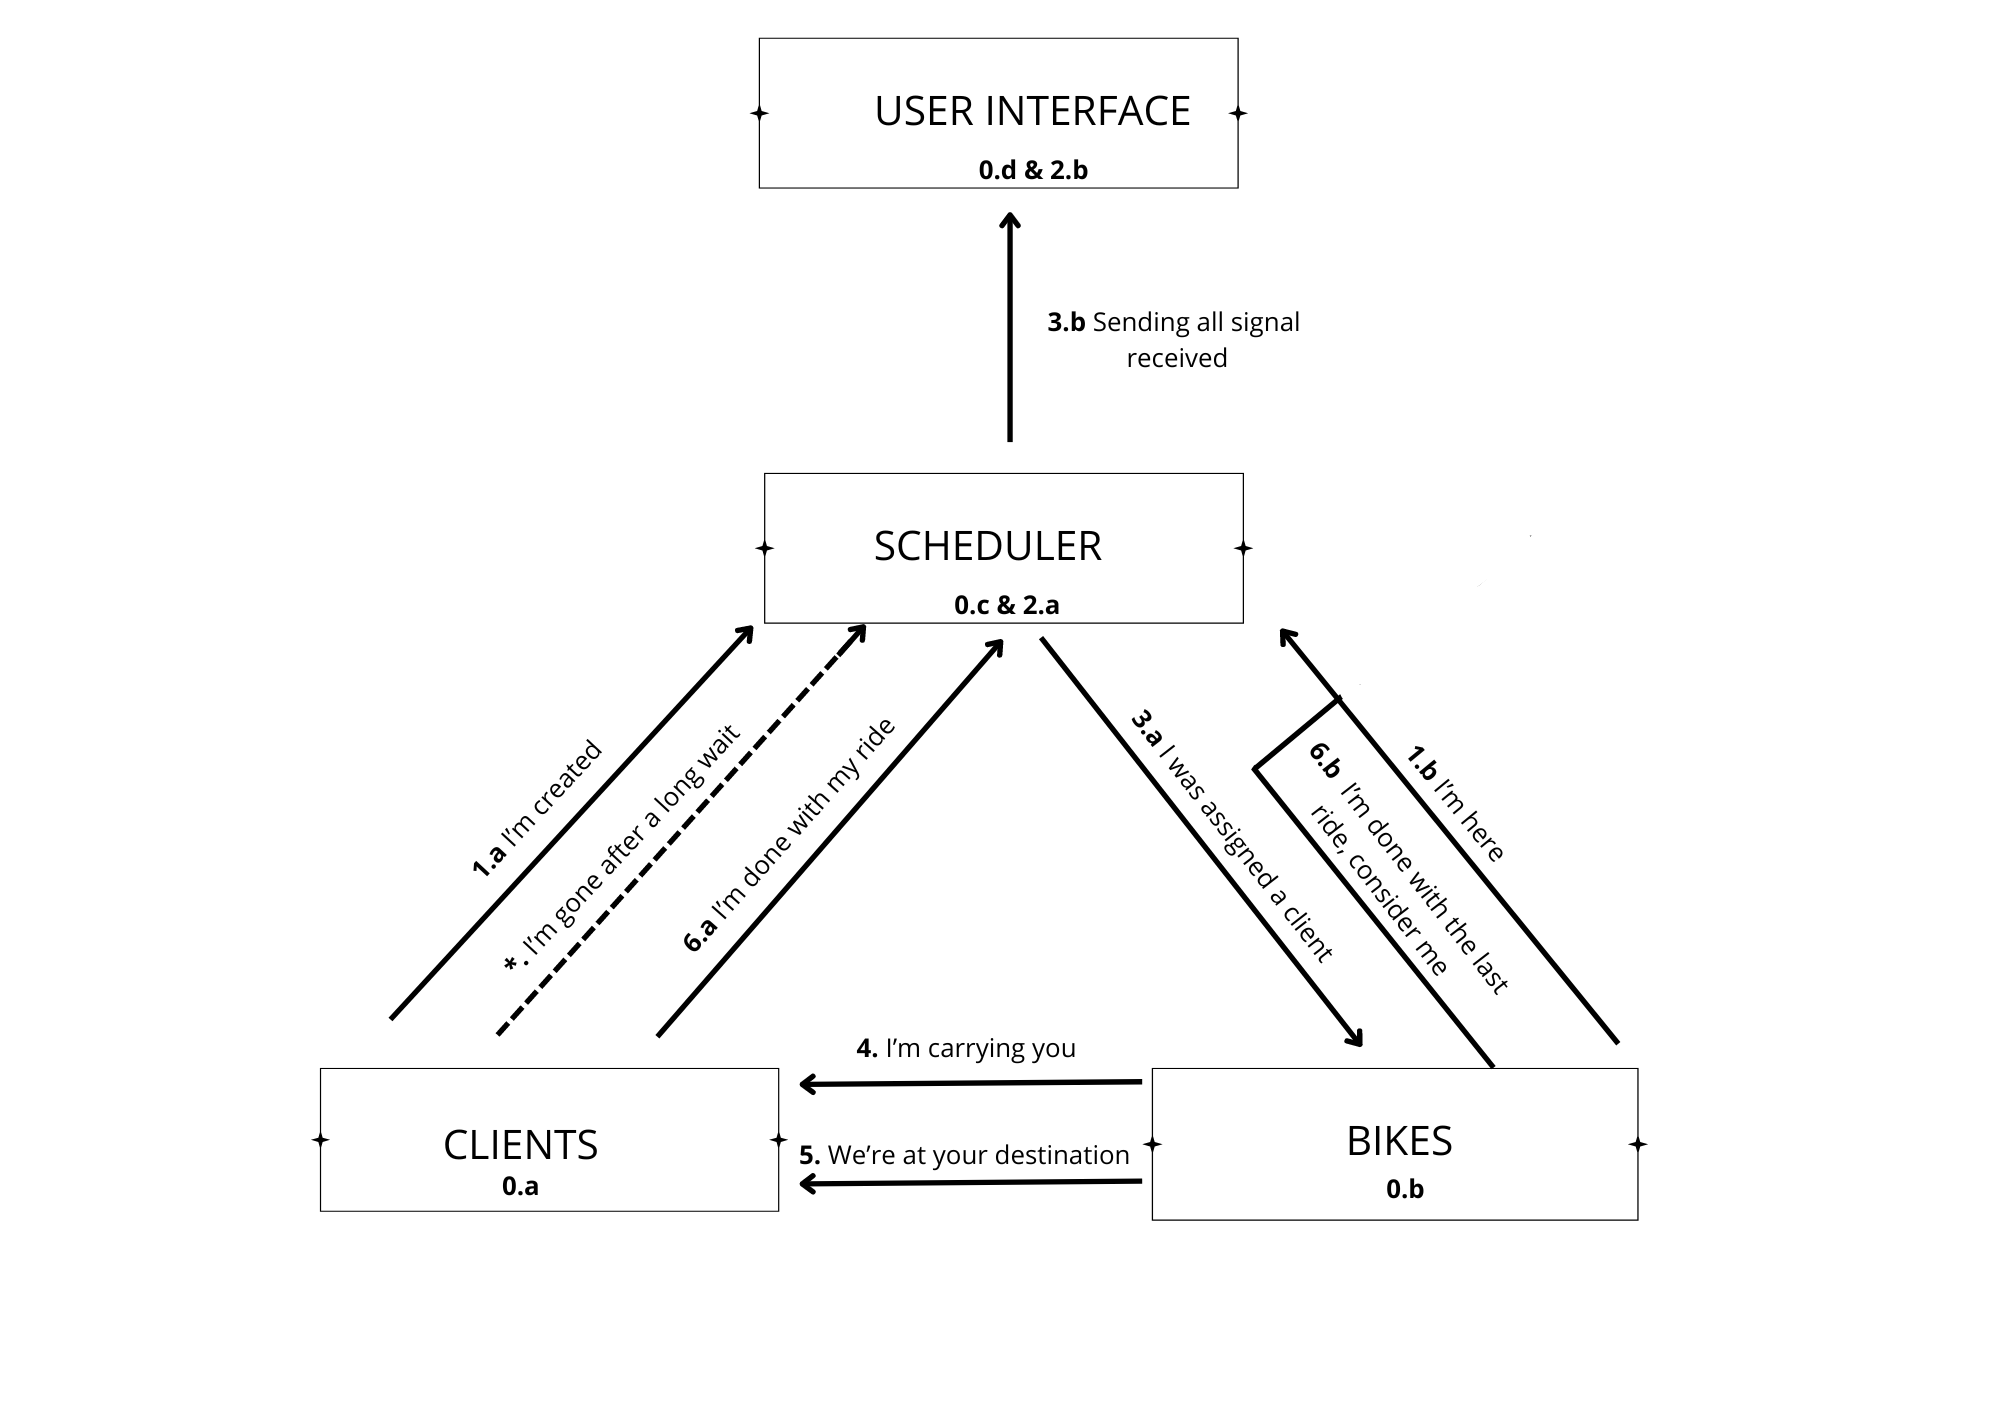
\includegraphics[width=1.0\linewidth]{Sections/Images/fro.png}
\end{center}

\newpage
\section{Implementation}

In this section, we will briefly outline the implementation of our solution using the C programming language.\\ We will start by presenting the different libraries, structures and data structures which will be used.To continue, discussing the \textbf{RPG}, then delve into the \textbf{clients}, \textbf{motorcycles}, and finally, the \textbf{scheduler}.\\
%-----------Structures explantion----------
\subsection{Differents libraries,structures and data structures}
    During the implementation of our program, different libraries, structures and data structures were used among which we can cite :

\subsubsection*{libraries}
The libraries we have utilized are:

\begin{itemize}
    \item \textbf{stdio.h} : Standard Input/Output operations.
    \item \textbf{stdlib.h} : General utilities, including memory allocation and conversion functions.
    \item \textbf{sys/types.h} : Definitions for various data types used in system calls.
    \item \textbf{sys/ipc.h} : Definitions for interprocess communication using IPC.
    \item \textbf{sys/shm.h} : Definitions and functions for shared memory operations.
    \item \textbf{sys/signal.h} : Definitions for signal handling.
    \item \textbf{sys/wait.h} : Declarations for wait functions.
    \item \textbf{math.h} : Mathematical functions.
    \item \textbf{unistd.h} : Standard symbolic constants and types, including functions like fork().
    \item \textbf{string.h} : String manipulation functions.
    \item \textbf{signal.h} : Signal handling functions.
    \item \textbf{stdbool.h} : Boolean data type and values.
    \item \textbf{sys/stat.h} : Declarations for functions and macros related to file status.
    \item \textbf{time.h} : Time-related functions.
    \item \textbf{glut.h} to make the user interface sing opengl functions 
\end{itemize}
\newpage
\subsubsection*{ structures and data structures}
   \begin{lstlisting}[style=customc, caption={quarter}]
  
    typedef enum QUARTER_YAOUNDE
{
    OMNISPORT,
    POLYTECH,
    TRAVAUX,
    .
    .
    .
    .
    ESSOS,
    NGOUSSO_1,
    QUARTIER_GENERAL,
    ECOLE_NORMALE,
    NKOA_BANG
} quarter;
\end{lstlisting}    
\begin{lstlisting}[style=customc, caption={client and bike}]
    typedef struct client
{
    /*
        Definition of a client type, which will references our process: one client is a process
        pid is the process id of the client (as we said, it's a process)
        start and dest are quarters, element of an enumeration of all quarters of our town
        price in an integer which represents the price that client will pay if there is a bic that drive him to his dest
    */
    pid_t pid;
    quarter start;
    quarter dest;
    unsigned int price;
    time_t wait_time;
} Client;
\end{lstlisting}
\newpage
 \begin{lstlisting}[style=customc, caption={bike}]
   
    /*
        Definition of a bike type, which will references our processes: one bi is a process
        pid is the process id of the bike (as we said, it's a process)
        itinerary is a table of  quarters, element of an enumeration of all quarters of our town
        
    */typedef struct Bike
{
   pid_t pid;
   int *itinerary;
}Bike;
 //type deque
typedef struct deque 
{   struct block *start;
    struct block *end;
}deque;

\end{lstlisting}

\begin{itemize}
    \item[\textbullet]The structure \textbf{quartier}: who does the correspondance between each quater and its Pid in the data structure
    \item[\textbullet] The structure \textbf{deque} :A deque, or double-ended queue, is a type of queue in which insertion and removal of elements can be performed from both the front and the rear. This means it does not follow the FIFO (First In First Out) rule.A deque provides more flexibility by allowing operations at both ends of the queue.
    \item[\textbullet] The strucure \textbf {Bike} : is one of the main structure of our program, the main ressource used in the program. This structure is defined as a type and its variables are : \begin{itemize}
        \item \textbf{It's PID} which is a unique number attributed to each bike after it's creation
        \item \textbf{It's Itinenary}: who defines the starting point of the bike and it's ending point.And we should note that an itinenary is a set of many destinations.
    \end{itemize}
    \item[\textbullet] The data structure \textbf{Quartier} : whose's role is to contain the name of all the quaters we will use to generate all the itinerary for our bike
\end{itemize}
\newpage

%---------RPG---------------------
\subsection{RPG (Random Process Generator)}
To implement this RPG, we will need   enter an infinite loop, representing the total duration of the program. At random intervals, we will simultaneously create processes representing motorcycles and customers. These processes will be modified in their operation using the \textbf{exec()} function.\\

The RPG, as defined earlier, is a program in which processes are created, representing either customers or motorcycles. After the creation of these processes, they will be directed to execute a binary file containing specific instructions that they will carry out.\\Here is the C code of the RPG code:%%%%%%%%%insérer le code ici%%%%%%%%%%%%

\begin{lstlisting}[style=customc, caption={  code of  RPG}]
#include <time.h>
#include <stdio.h>
#include <unistd.h>
#include <stdlib.h>
#include <sys/types.h>
#define MAX_SLEEP_TIME 2
#define CLIENT_GENERATION_FREQ 2

int main(int argc, char *argv[])
{
    srand(time(NULL));
    int balance = 0;
    while (1)
    {
        pid_t pid = fork();
        if (pid == -1)
            fprintf(stderr, "Error, cannot start neither bike or client process\n");

        if (pid == 0)
        {
            if (balance % 2)
            {
                char* args[] = {"../../client/bin/client.out", argv[1], NULL};
                execvp("../../client/bin/client.out", args);
            }
            else
            {
                char* args[] = {"../../moto/bin/bike.out", argv[1], NULL};
                execvp("../../moto/bin/bike.out", args);
            }
        }

        balance++;
        sleep(5);
    }

    return 0;
}


\end{lstlisting}

This program continuously creates processes at random intervals less than a given time T, which is a compilation parameter. Subsequently, it modifies their instructions using the \textbf{execvp()} function.using the variable balance,it create clients and bikes.

\newpage
%--------------------------------------

%-------------Client---------------------
\subsection{Clients}
To implement the client, let's describe how to carry out each task.\\ The following provides an overview of how the client operates.\\

When creating a motorcycle, the following steps are taken:
\begin{enumerate}
  \item \textbf{Information Generation}: Here, we use the \textbf{random();} function to generate the client's starting and ending destinations. The PID is retrieved using the \textbf{getpid();} function.\\
  \begin{lstlisting}[style=customc, caption={random and pid functions}]
\\random function()
#include <stdlib.h>
long int random(void);

\\getpid()
#include <sys/types.h>
#include <unistd.h>
pid_t getpid(void);


\end{lstlisting}


  \item \textbf{Shared Memory Segment Creation}: We create using the \textbf{shmget();} function and attach using the \textbf{shmat();} function.
    \begin{lstlisting}[style=customc, caption={shmget and shmat functions}]
\\shmget function()
#include <sys/shm.h>
int shmget(key_t key, size_t size, int shmflg);

\\shmat()
#include <sys/shm.h>
void *shmat(int shmid, const void *shmaddr, int shmflg);
\end{lstlisting}


  \item \textbf{Signal Transmission to Scheduler}: It then sends a signal to the scheduler informing the completion of the initial part execution, this using the \textbf{kill();} function.\\
    \begin{lstlisting}[style=customc, caption={kill function}]
\\kill fuction()
#include <signal.h>
int kill(pid_t pid, int sig);

\end{lstlisting}


  \item \textbf{Signal Waiting}: It waits for the scheduler's signal, which continues until it reaches its limit using the \textbf{sleep();} function. If the allocated time is exceeded, the process is then terminated, a signal is sent to the scheduler, and it is removed from the list of clients using the \textbf{kill();} and \textbf{SIGNAL(int,void*);} functions.\\
  \newpage
    \begin{lstlisting}[style=customc, caption={sleep and signal functions}]
\\sleep fuction()
#include <unistd.h>
unsigned int sleep(unsigned int seconds);
\\SIGNAL()
void (*signal(int sig, void (*func) (int))) (int);

\end{lstlisting}

  

  \item \textbf{Signals Reception by the Client}: It receives a signal from the bike informing that it has been transported. At the end of the ride, it receives a signal from the bike indicating the end of the ride and terminates. This is done using the \textbf{SIGNAL} function, and it concludes with \textbf{exit(0)} if the client is dissatisfied and \textbf{exit();} if satisfied.
\end{enumerate}
\newpage
%------------------------------------------


%-------------Bike Section---------------------
\subsection{Bike}
The bike entity is defined by a data structure of \textbf{type def struct bike }which has its pid and itinerary as data. Its itinerary is itself an array formed of five consecutive elements from the list of neighborhoods chosen randomly.\\ To implement the Bike, we will follow the steps below:

\begin{enumerate}

    \item \textbf{Bike Creation }:In this step we start by allocating memory space to create the bike using the \textbf{malloc();} function. Then, the bike is initialized from a start point randomly chosen from the list of neighborhoods and incrementing the list of neighborhoods until we have five neighborhoods. The pid of the bike is retrieved using the \textbf{getpid();}function. All this bike creation is done using a function called \textbf{BikeCreation();} of type void and returns an element of type bike.% ici il y'a une impossibilité de pouvoir mettre le tiret de 8 car il faut respecter un certain encodage.
   
   \item \textbf{Shared Memory Segment Creation }: In this segment, the bike creates a shared memory segment using the \textbf{shmget();} function and attaches it using the \textbf{shmat();} function. In this segment, the bike writes its itinerary using the \textbf{memcpy();} function.
   
    \item \textbf{Signal Transmission to Scheduler}: The bike then sends a bike created signal to the scheduler using the \textbf{kill();} function. % ici il y'a une impossibilité de pouvoir mettre le tiret de 8 car il faut respecter un certain encodage.
    
    \item \textbf{Signal Waiting} : After sending its signal, the bike waits for a while using the \textbf{sleep();} function. A handler will be in charge of transmitting the Central Scheduler signal when the time comes.
  
   \item \textbf{Signal Transmission to Client} : Here, the bike reads the client’s pid in the shared memory segment and sends a signal to the client to say “I have accepted you” using the \textbf{kill();} function. Then, the process starts over.

\end{enumerate}
		

\newpage
\begin{lstlisting}[style=customc, caption={ Bike creation}]
#include "../headers/defines.h"
#include "../headers/signal.h"
#include "../headers/initialisation_bikes.h"

char *quartier[111] = {"Centre commercial","Elig Essono","Etoa MekiI","Nlongkak",... ,"Minkoameyos","Nkolso"
};
// Return a bike filled with his parameters
Bike *create_bike(){
    Bike *bike = (Bike*)malloc(sizeof(Bike));

    // if alloc fails
    if(!bike) return NULL;

    // Generating a itinerary filled with a random of 5 consecutives quarters
    int start = random_integer(0, NB_QUARTER - RADIUS); 
    int* itinerary = (int*)malloc(sizeof(int) * RADIUS);
    
    // Filling consecutives quarters
    for (int i = 0; i < RADIUS; i++)
        itinerary[i] = start++;

    // Filling the new bike structure
    bike->pid = getpid(); // Getting pid process
    bike->itinerary = itinerary;

    return bike;
}
void write_infos_bike(Bike *bike){
    memcpy(shm_zone, bike, sizeof(Bike));
}

\end{lstlisting}

%\newpage

\begin{lstlisting}[style=customc, caption={ Shared memory segment creation}]
void create_segment(pid_t pid){
    shm_id = shmget((key_t)pid, SEG_SIZE, IPC_CREAT | IPC_EXCL | S_IRUSR | S_IWUSR);
    shm_zone = shmat(shm_id, NULL, 0);
}
\end{lstlisting}

\newpage
\begin{lstlisting}[style=customc, caption={ signals (transmission to scheduler , waiting , transmission to client)}]

#include "../headers/defines.h"
#include "../headers/signal.h"
#include "../headers/initialisation_bikes.h"

// Generate a random integer between a and b included
int random_integer(int a, int b){
	return (rand() % (b - a + 1)) + a;
}
void starting_course(pid_t client_pid){
	kill(client_pid, STARTED_COURSE);
}
void ended_course(pid_t client_pid){
	kill(client_pid, ENDED_COURSE);
}

// Receive a signal of client and read in the shm the pid of client and change a statut of moto
void bike_handler(int signum){
	if(signum != SEGMENT_READY)
		return;

	pid_t client_pid = *((pid_t*)shm_zone);
	// Send a signal to precise that we are carrying a client
	starting_course(client_pid);
	// Time interfal for the course
	sleep(random_integer(TASK_TIME_MIN, TASK_TIME_MAX)); 
	// Send a signal to precise that we have ended the course
	ended_course(client_pid);
	// Write again bike's infos
	write_infos_bike(bike);
	// Resend the signal to the CS
	send_signal(oc_pid, BIKE_CREATED);
}
// Atttach functions to signal
void set_handler(){
	signal(SEGMENT_READY, &bike_handler);
}
// Send signal to CS 
void send_signal(pid_t oc_pid, int sig){
	kill(oc_pid, sig);
}
\end{lstlisting}
\newpage
%--------------------------------------

%-----------Central Schedular------------
\subsection{Central Scheduler}
To implement our scheduler,we are going to present step by step,the following ideas:
\begin{enumerate}
  \item \textbf{Data initialization}:Here we start by creating two deques one for the clients and another one for the bikes which are present. And then arm the different signal handlers.
   \begin{lstlisting}[style=customc, caption={creation of deques}]
// client_deque and bike deque
 /* @brief Create a deque object
 * @return deque* deque created
 */
deque *create_deque()
{   deque *new_deque = (deque *)malloc(sizeof(deque));
    if (new_deque == NULL) 
    {
        perror("Error, canot create deque\n");
        exit(EXIT_FAILURE);
    }
    new_deque->start = NULL;
    new_deque->end = NULL;
    return new_deque;
}
void init_deques()
{   bikes_deque = create_deque();
    clients_deque = create_deque();
}
//type deque
typedef struct deque 
{   struct block *start;
    struct block *end;
}deque;

\end{lstlisting}
  
  \item \textbf{Listening Mode}: The Scheduler now listens to various signals from bikes and clients for a set time t.\\
The different signals awaited are: \textbf{CLIENT-CREATED} and \textbf{BIKE-CREATED}.\\We perform the waiting using the \textbf{signal()} function. We use handlers to process these different signals with \textbf{sig-actions}

  \item \textbf{Masking of signals}: After the said time, the signals sent as of now are not taken into consideration for the following scheduler operations.
  
  \item \textbf{Saving Clients}: It saves the different clients into the deque saving it using the FIFO policy and same is done for the different bikes using the other deque.
  
  \item \textbf{Assigning Clients to Bikes}: Using the first fit protocol, the various clients are assigned to the available bikes and for this to happen, a signal is sent(with the function \textbf{kill();} ) to the chosen bike and the chosen client is removed from client deque.
  
  \item \textbf{Restart}: The procedure then restarts from the listening period and the masked items are added to the appropriate deques.
\end{enumerate}
%--------------------------------------------

%------------Graphical Interface-------------
%\subsection{Graphical Interface}

%--------------------------------------------
\newpage
\section{User Interface}
To implement the interface of this project, we have opted to utilize the \textbf{OpenGL} library in the C programming language. This library proves to be highly advantageous for crafting interactive interfaces. In order to carry out this task systematically, we have chosen to break down the responsibilities into several key modules: the \textbf{Central Scheduler (CS)}, the \textbf{User Interface (UI)}, and the \textbf{Client} and {Bike} modules. This modular approach ensures effective management of each aspect of the interface, ensuring a robust design and smooth development.

Furthermore, we will facilitate interaction among these different modules through interprocess communication and the use of shared memory segments. In the following sections, we will provide a detailed explanation of the work accomplished in each module and illustrate the results.


%\begin{center}
 %   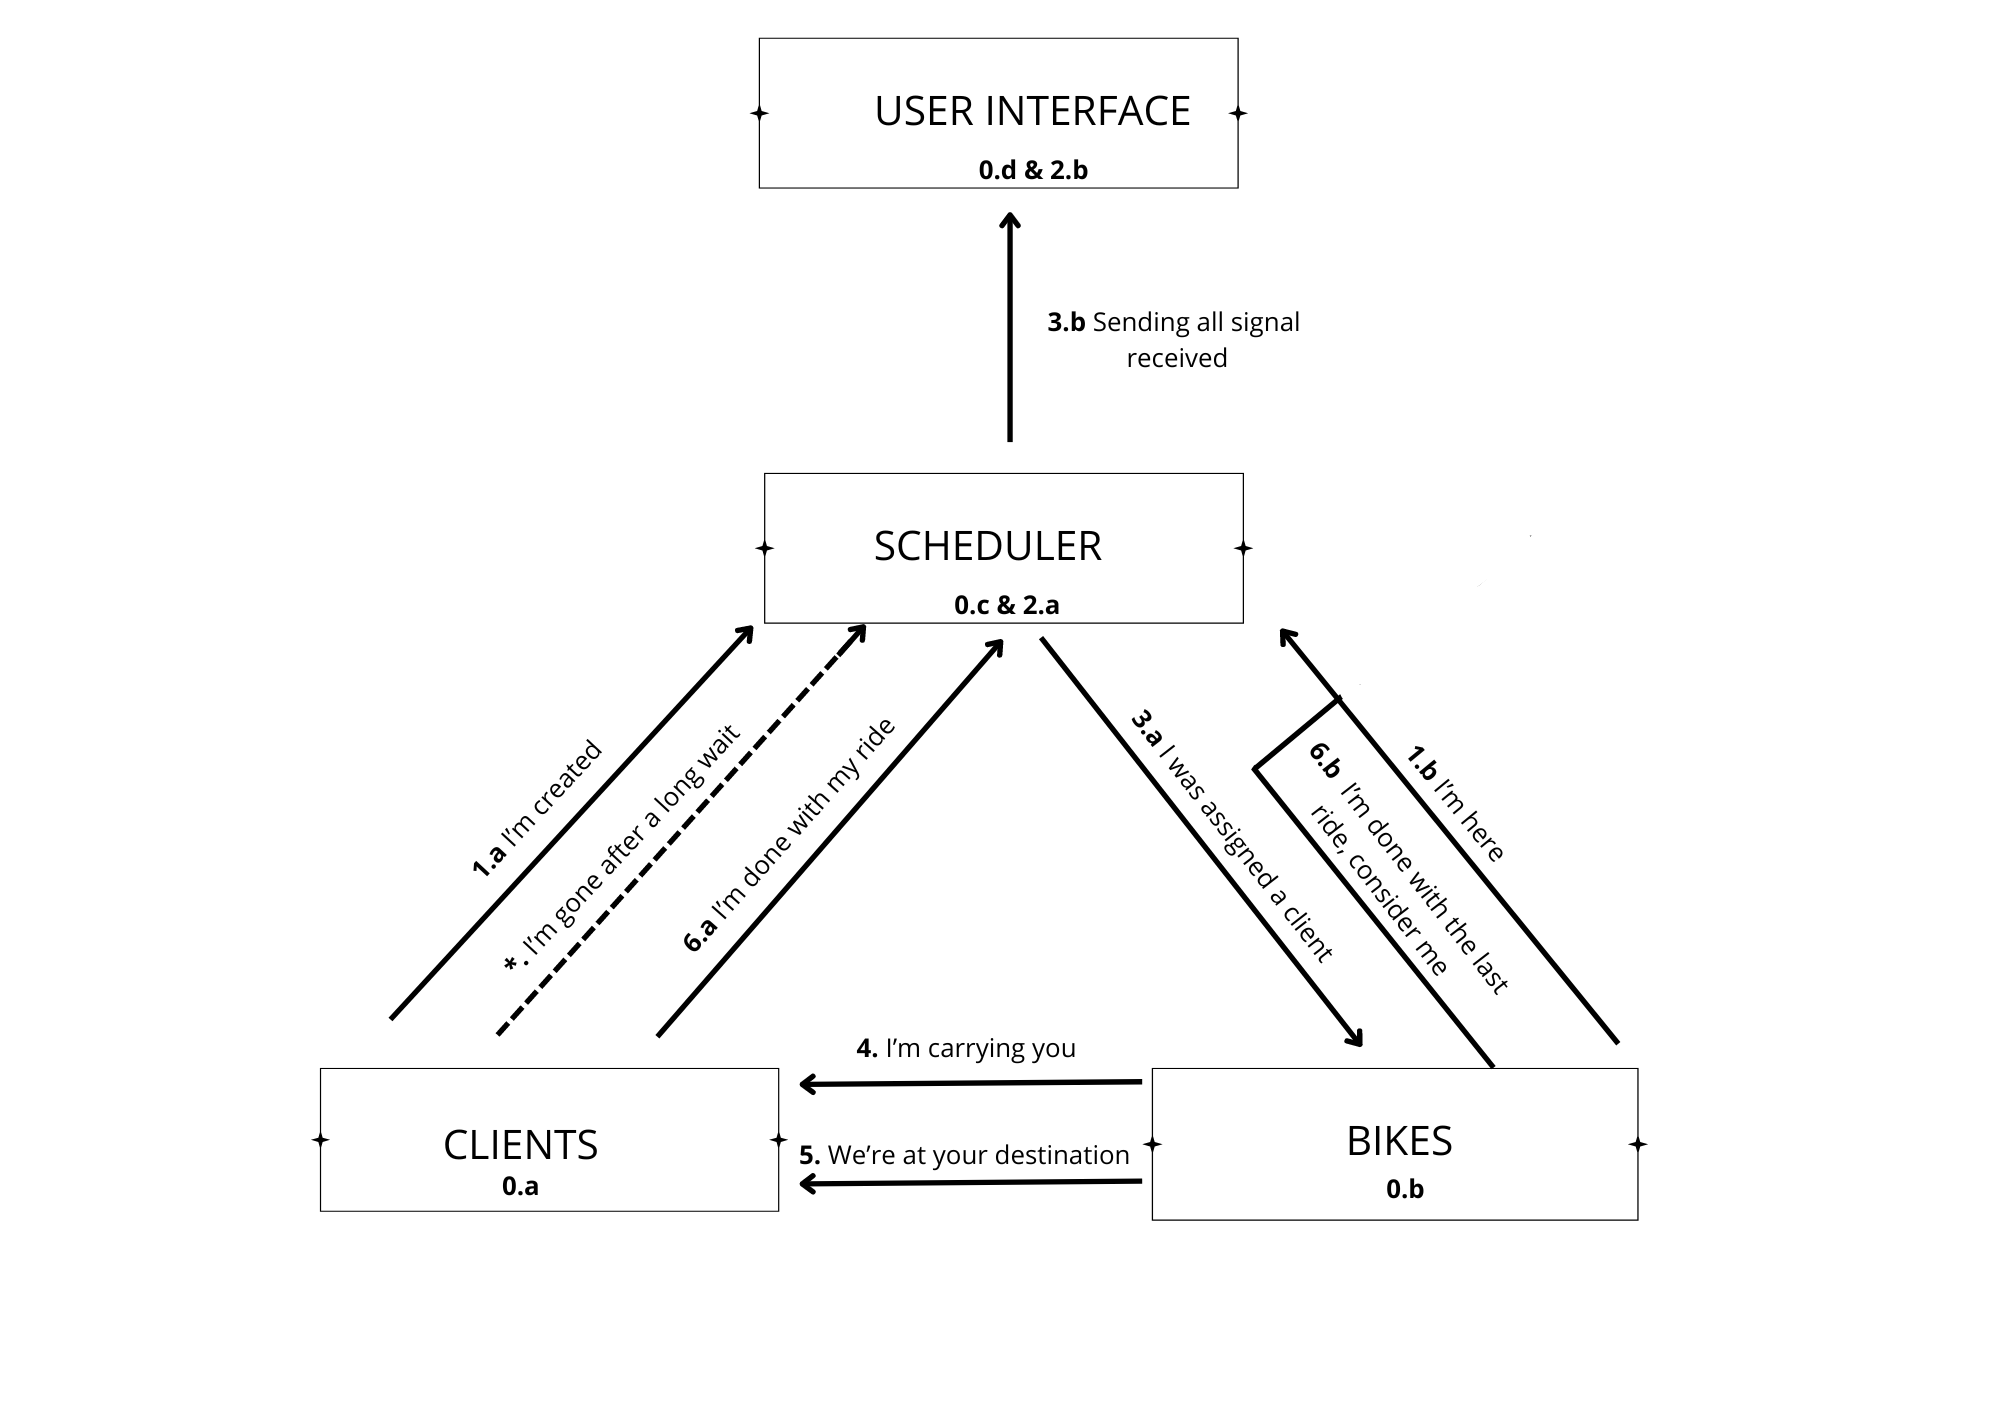
\includegraphics[width=0.7\linewidth]{Sections/Images/fro.png}
%\end{center}




The following figure gives a brief summary of all what has been explicated above.
The numbered sections 0.a, 0.b, 0.c, 0.d, 2.a and 2.b which couldn't be further explained on the figure respectively represent the following:

\begin{enumerate}
  \item \textbf{Step 0.a}:This represents the information generation and the shared memory segment creation.
  \item \textbf{Step 0.b}: This represents the route and the shared memory segment creation.
  \item \textbf{Step 0.c}: This part is concerned with the data initialization and listening mode from the scheduler
  \item \textbf{Step 0.d}: This part is concerned with the initialization of the user interface
  \item \textbf{Step 2.a}: This part is concerned with the different saving of the different bikes and clients information.
  \item \textbf{Step 2.b}: This part is concerned with the the treatment of all the various signals by the user interface.
\end{enumerate}
%-----------------------------------------
\begin{center}
   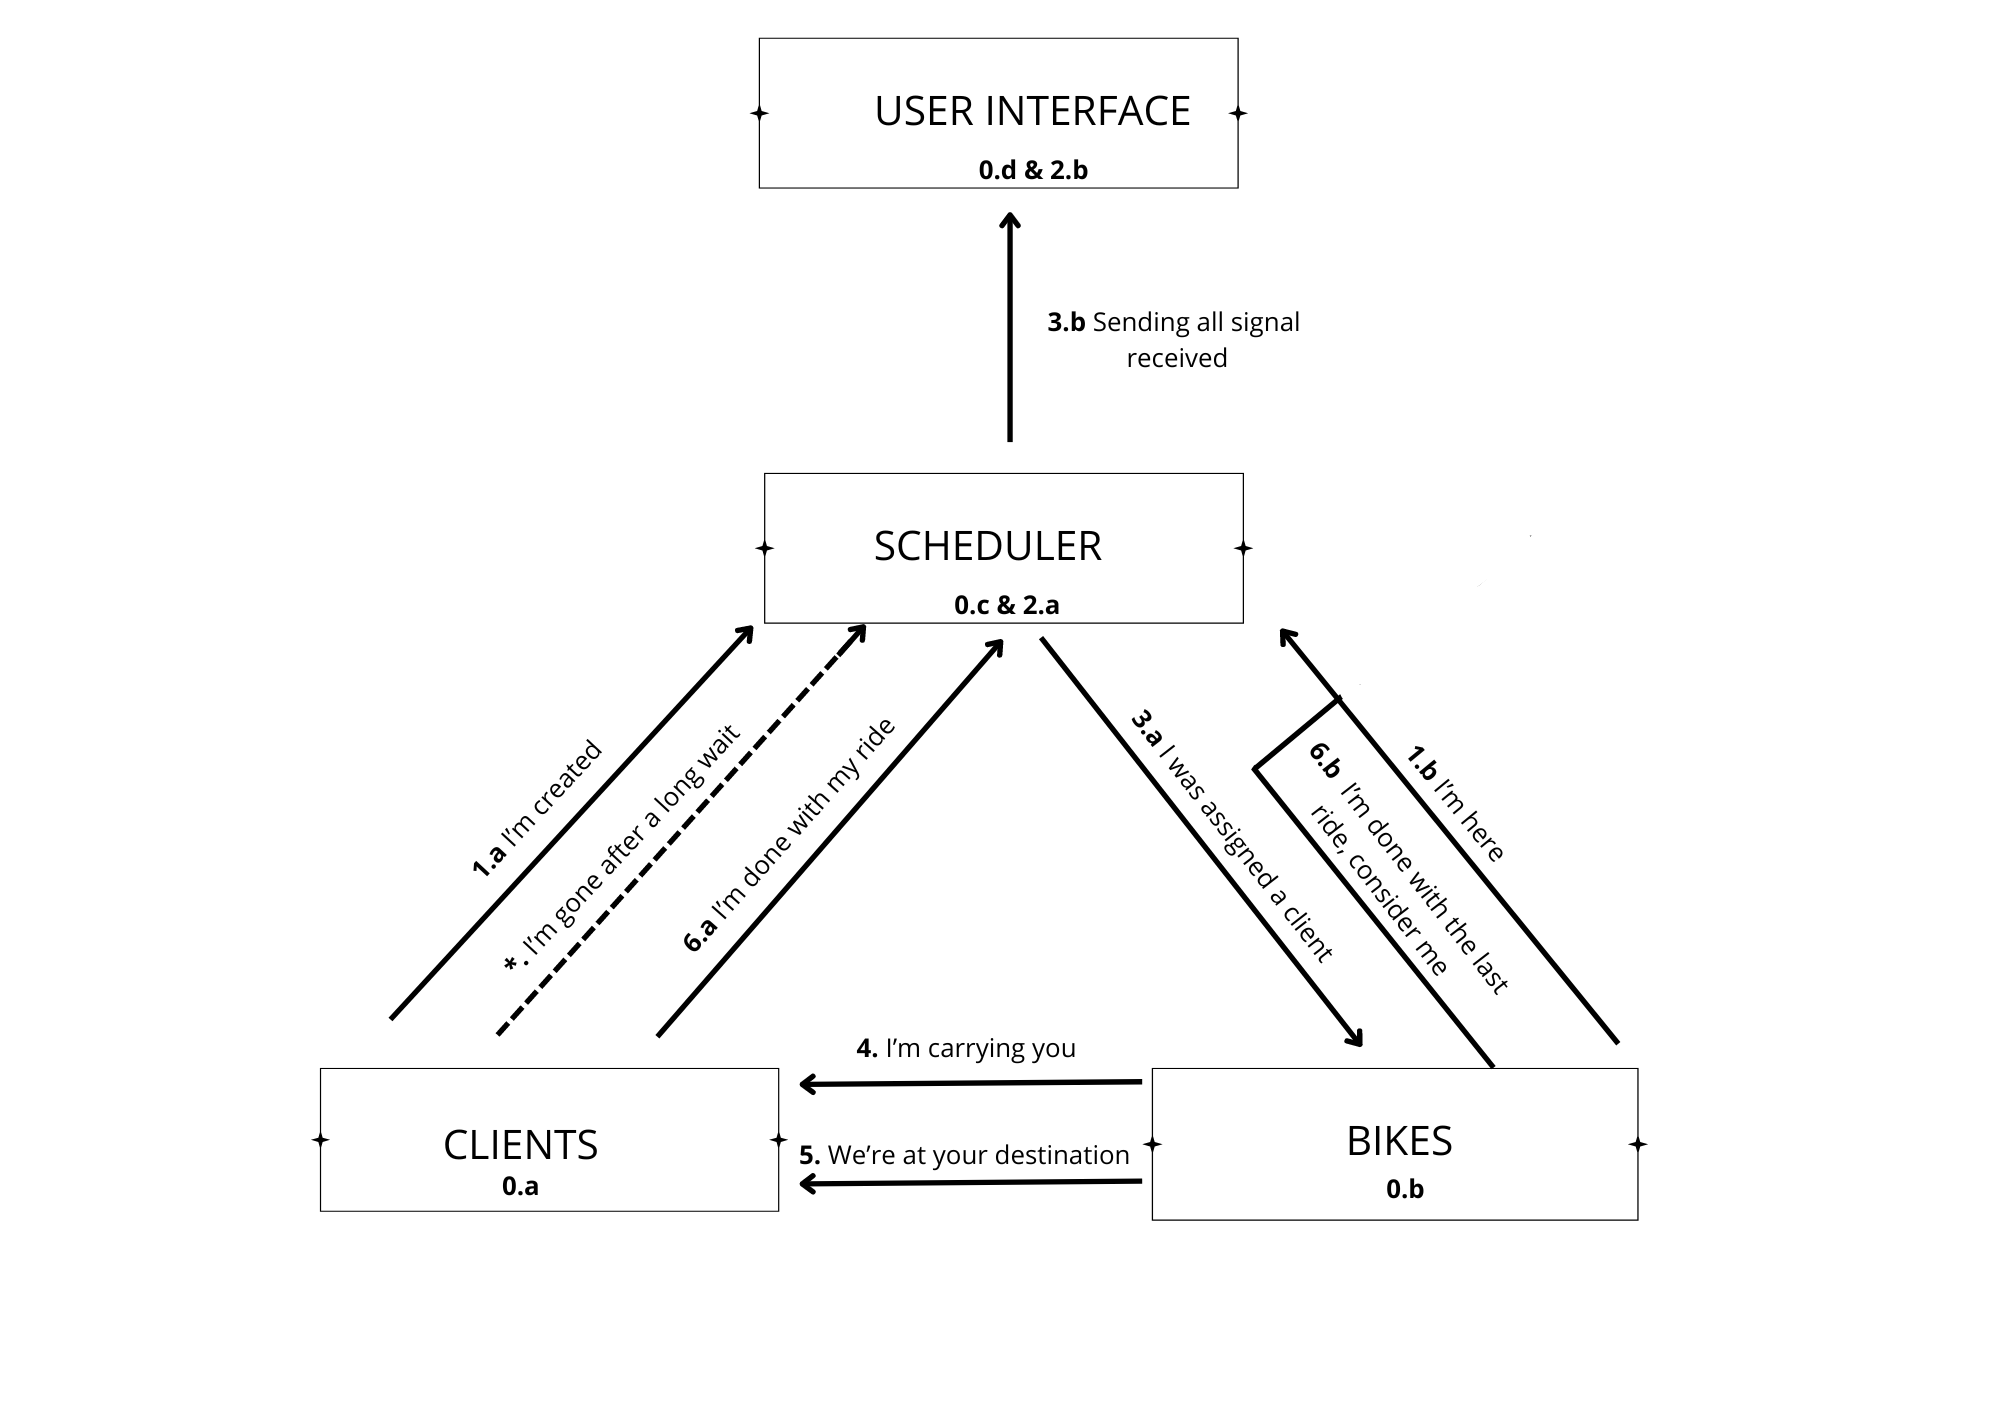
\includegraphics[width=0.7\linewidth]{Sections/Images/fro.png}
\end{center}


\newpage
\subsection{Client and bike}
Graphical clients and motorcycles are simply defined using G-client and G-bike data structures described below.
 \begin{lstlisting}[style=customc, caption={structures for user interface}]
#include <unistd.h>

// 2D point structure
typedef struct Point
{
    float x;
    float y;
}Point;

//client's structure
typedef struct G_client
{
    float radius;
    Point* start;
    Point* dest;
    Point* center;
}G_client;

//bike's structure
typedef struct G_bike
{
    float side;
    Point* start;
    Point* center;
}G_bike;


typedef struct G_quarters 
{
    int id;
    Point *loc;
} G_quarters;


typedef struct G_data
{
    pid_t bike_pid, client_pid;
    int bike_start;
    int client_start, client_dest;

    struct G_data* next;   
}G_data;
\end{lstlisting}
We also define G-quarters structures to describe the graphic area and G-data to link a motorcycle to a client it must go to. This structure will be useful to ensure the simultaneous movement of our motorcycle and client on the interface.
\newpage
\subsection{Scheduler}
The central scheduler operates in this section regarding communication with the background of our project. In fact, it is responsible for informing the interface process about the pairs $(client, motorcycle)$ that need to be moved. It writes this information into a shared memory segment obtained through the \textbf{shmget()} function and sends a signal to the UI using the \textbf{kill()} function. The UI will then read the information from the shared memory segment and use it to simultaneously move both the motorcycle and the client it carries. The information written includes:
\begin{enumerate}
    \item the client's process ID (pid)
    \item the motorcycle's process ID (pid)
    \item the starting and destination points of the client
\end{enumerate}
The UI will then use this data to carry out the movement.

%After we have recovered the user's interface Pid, we will use it to get the scheduler's PId. This is the command to launch this :\\

%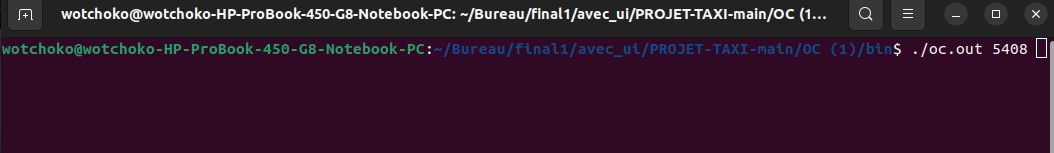
\includegraphics[width=1.0\textwidth]{Sections/Images/oc-out.png}\\

%And this is the result of this command :\\

%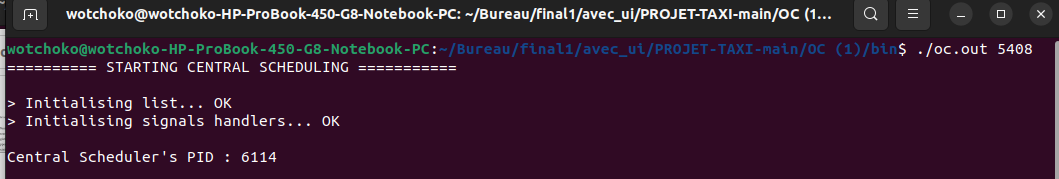
\includegraphics[width=1.0\textwidth]{Sections/Images/oc_pid.png}\\
\newpage
\subsection{UI}
Just as in the scheduler, the UI needs a few data structures to store the information of the clients and motorcycles it needs to display.
\begin{itemize}
    
    \item First, it maps each neighborhood from the backend, stored as an integer, to a graphical neighborhood defined by the G-quar structure mentioned above.
    \item Then, it needs a named list of pairs \texbf{list-t} 
    $(client,moto)$ during display.
\end{itemize}
The UI also needs certain functions to perform its task:
\begin{enumarate}
    \item The function \textbf{init-list()} creates the couple's list $(client,moto)$ for data storage.
    \item The function \textbf{init-quarters-list()} is in charge of creating a correspondence between the quarters back-end and the quarters on the interface and then store it in the quarter-list data structure.
    \item The function \textbf{get-quarter-pos} which allows obtaining the graphical position of a neighborhood based solely on its PID. In fact, it will search the neighborhood list to accomplish this. It returns a graphical point.
    \item A handler \textbf{handle-oc-scheduled} which is used after each scheduling by the scheduler. It allows the UI to read the shared memory segment with the scheduler and retrieve the necessary information to move a pair. $(client,moto)$
    \item The UI also requires specific functions to draw the clients and motorcycles, which we do not consider necessary to list here. Just note that the motorcycles will be represented as squares, while the clients will be represented as circles on the screen.
\end{enumarate}
Here are the function signatures for these functions:
%stp nina regarde uneu ledernier commentaire ans le bloc de code ci-dessous j'arrive pas à bbien formuler.celui du handle%
\newpage
\begin{lstlisting}[style=customc, caption={functions of UI}]
/**
 * @brief initialize bikes and clients tuple list
 * 
 */
void init_list(void)
{
    bikes_n_clients_list = create_list();
}
/** 
 * @brief Function to create many points for display and store them in a list_quarter. 
 * 
 */
void init_quaters_list() 
/**
 * @brief Function to find the coordinates of a quarter based on its ID. 
 * @param id(int) 
 * @return point 
 */
Point* get_quater_pos(int id)
/**
 * @brief handle is used to gather information about couple client-bike which now moves together. 
 * @param signum(int) is a number of signals used to call this handler
 * @param *info(siginfo_t) helps to gather information for the the handle
 * @param *context is of type void 
 */
void handle_oc_scheduled(int signum, siginfo_t *info, void *context)

\end{lstlisting}\newpage
\newpage
\section{Test and evaluation}

%-----------Without interface--------------------
\subsection{without interface}

\subsubsection{scheduler}
\begin{figure}[H]
    \centering
    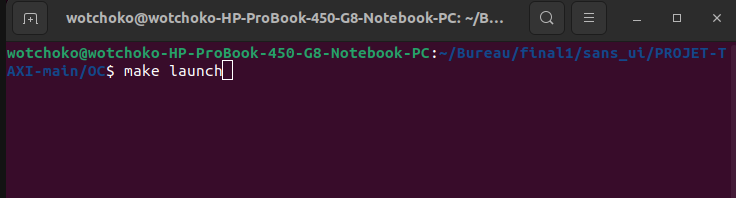
\includegraphics[width=1.0\textwidth]{Sections/Images/new_images/b1.png}
    \caption{compiling scheduler only}
    \label{fig:enter-label}
\end{figure}
\begin{figure}[H]
    \centering
    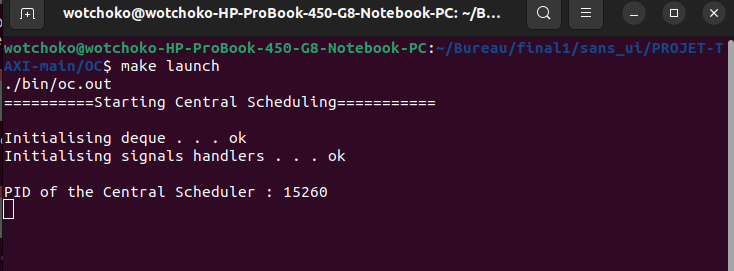
\includegraphics[width=1.0\textwidth]{Sections/Images/new_images/c1.png}
    \caption{result}
    \label{fig:enter-label}
\end{figure}

\begin{figure}[H]
    \centering
    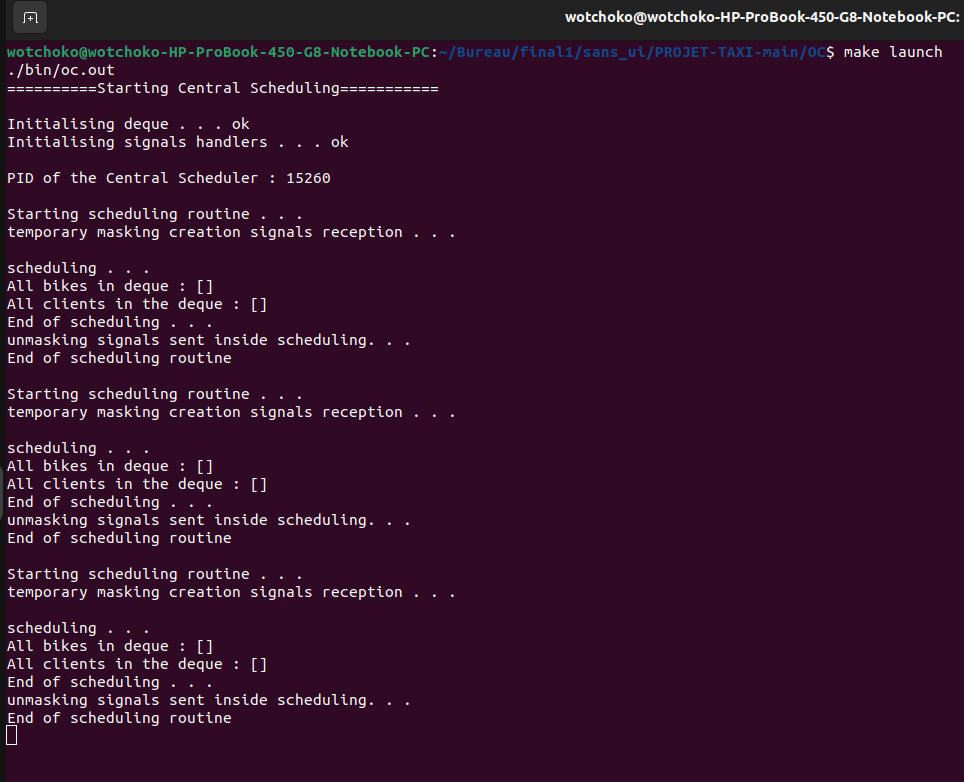
\includegraphics[width=1.0\textwidth]{Sections/Images/new_images/c2.png}
    \caption{we see that deques are empty because clients and bikes are not created.Now we are going to compile it with RPG}
    \label{fig:enter-label}
\end{figure}
\subsubsection{scheduler with RPG}

\begin{figure}[H]
    \centering
    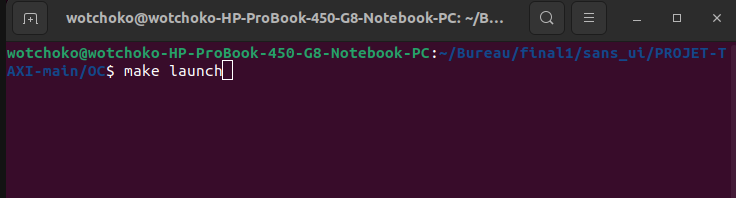
\includegraphics[width=1.0\textwidth]{Sections/Images/new_images/b1.png}
    \caption{to compile OC again}
    \label{fig:enter-label}
\end{figure}

\begin{figure}[H]
    \centering
    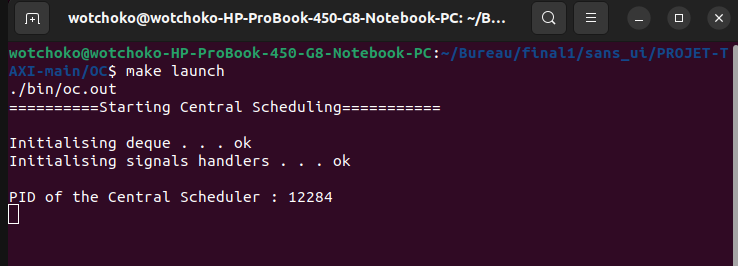
\includegraphics[width=1.0\textwidth]{Sections/Images/new_images/b2.png}
    \caption{new result before RPG}
    \label{fig:enter-label}
\end{figure}

\begin{figure}[H]
    \centering
    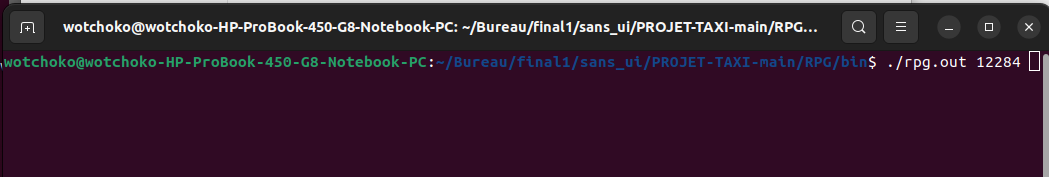
\includegraphics[width=1.0\textwidth]{Sections/Images/new_images/b3.png}
    \caption{to compile RPG with pid of scheduler}
    \label{fig:enter-label}
\end{figure}

\begin{figure}[H]
    \centering
    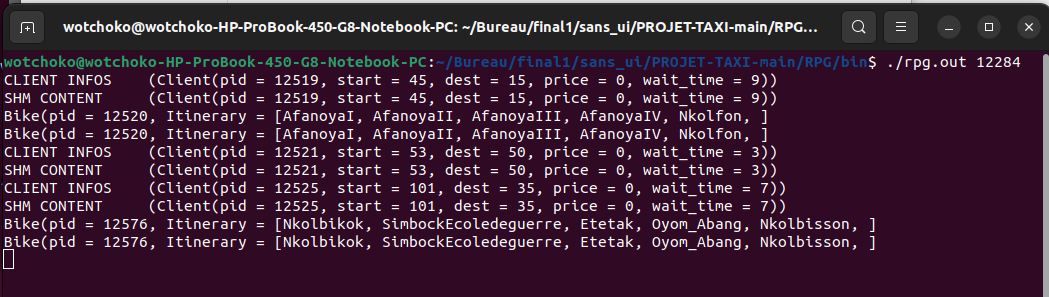
\includegraphics[width=1.0\textwidth]{Sections/Images/new_images/b4.png}
    \caption{result in RPG}
    \label{fig:enter-label}
\end{figure}
% \begin{figure}[H]
%     \centering
%     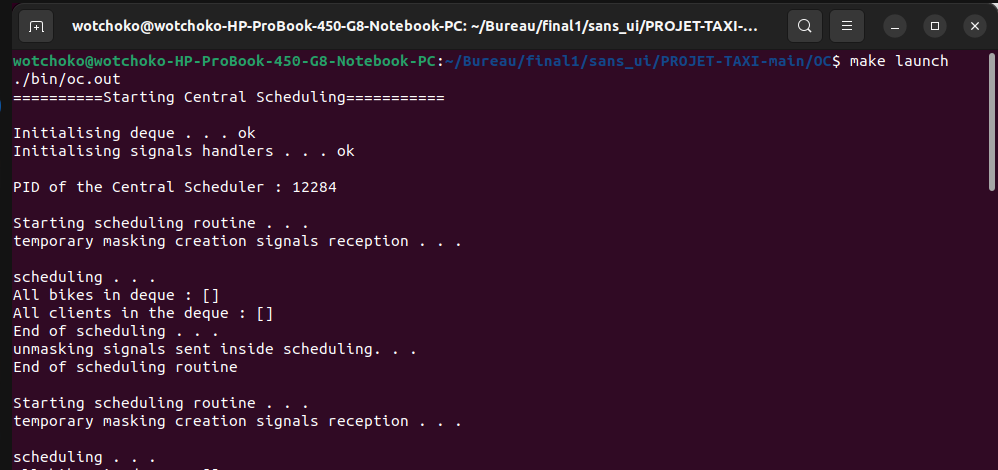
\includegraphics[width=1.0\textwidth]{Sections/Images/new_images/b5.png}
%     \caption{result in RPG}
%     \label{fig:enter-label}
% \end{figure}

\begin{figure}[H]
    \centering
    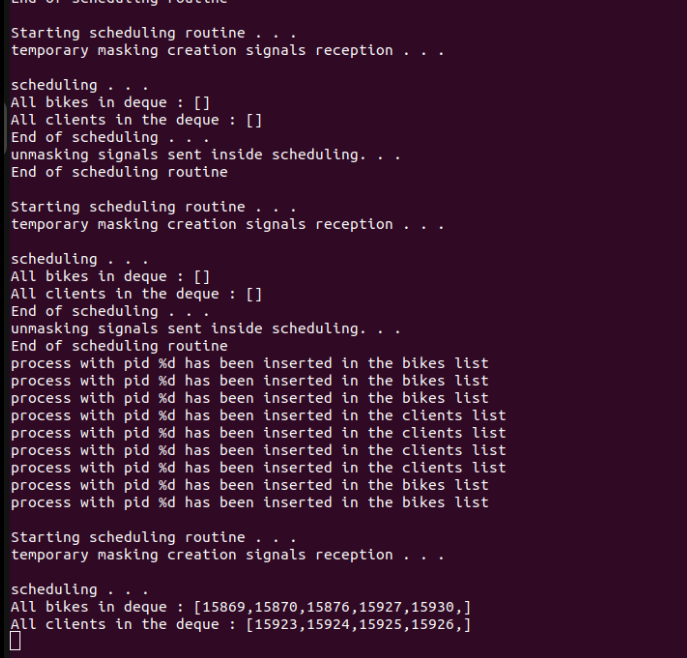
\includegraphics[width=1.0\textwidth]{Sections/Images/new_images/b66.png}
    \caption{scheduling}
    \label{fig:enter-label}
\end{figure}










%-----------With interface-------------

\subsection{with interface}

\begin{figure}[H]
    \centering
    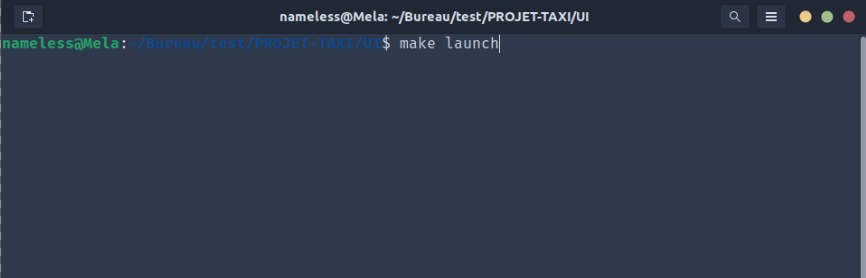
\includegraphics[width=1.0\textwidth]{Sections/Images/new_images/a100.png}
    \caption{compiling of UI}
    \label{fig:enter-label}
\end{figure}

\begin{figure}[H]
    \centering
    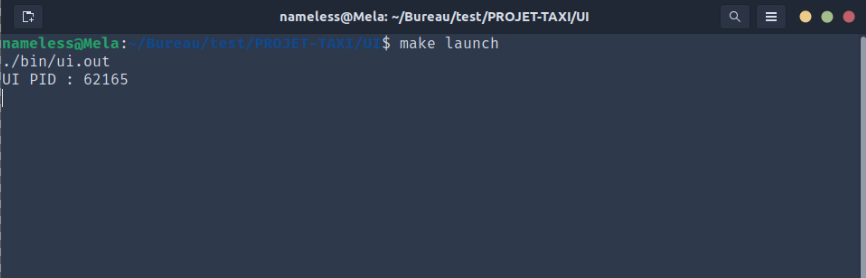
\includegraphics[width=1.0\textwidth]{Sections/Images/new_images/a200.png}
    \caption{result of compiling UI in terminal }
    \label{fig:enter-label}
\end{figure}
\begin{figure}[H]
    \centering
    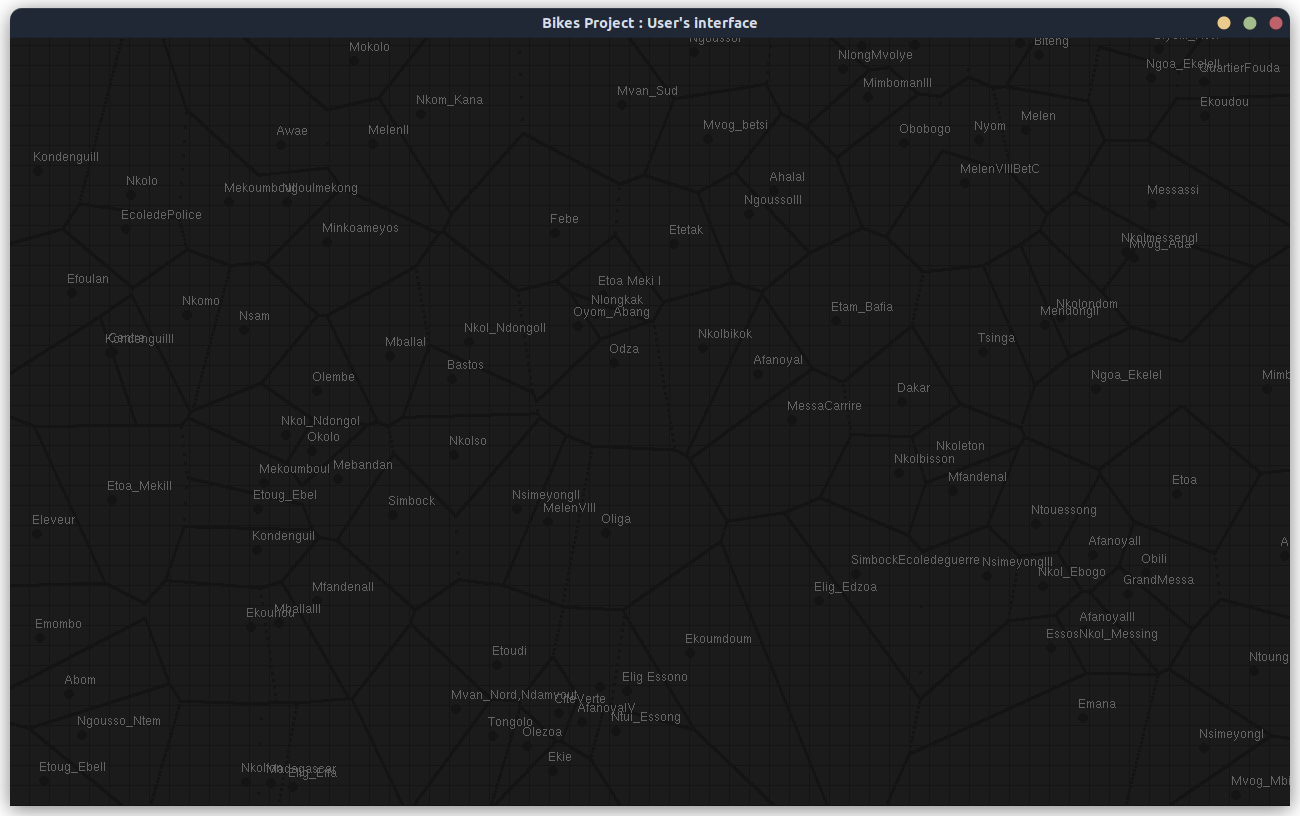
\includegraphics[width=1.0\textwidth]{Sections/Images/new_images/a3.png}
    \caption{result of compiling UI}
    \label{fig:enter-label}
\end{figure}

% \begin{figure}[H]
%     \centering
%     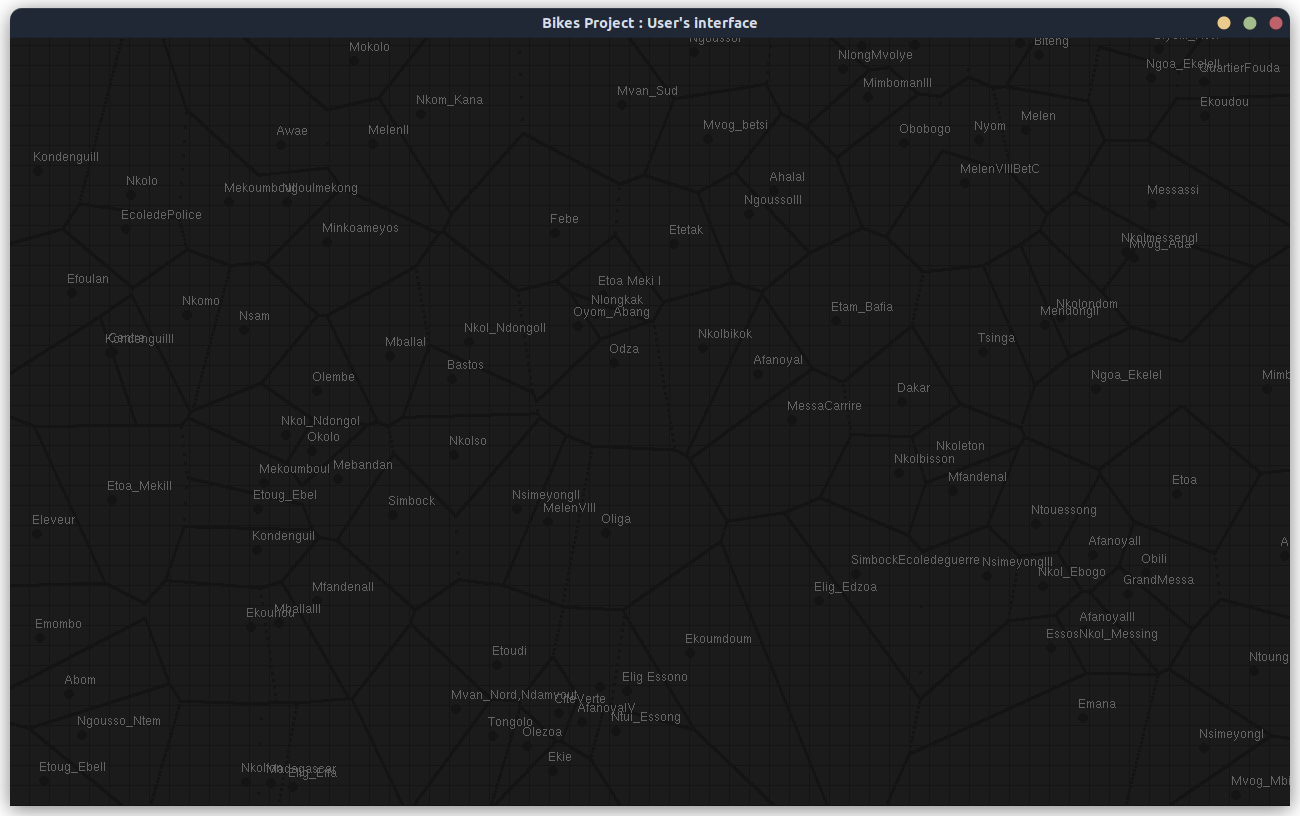
\includegraphics[width=1.0\textwidth]{Sections/Images/new_images/a3.png}
%     \caption{compiling of OC with the pid of UI}
%     \label{fig:enter-label}
% \end{figure}

\begin{figure}[H]
    \centering
    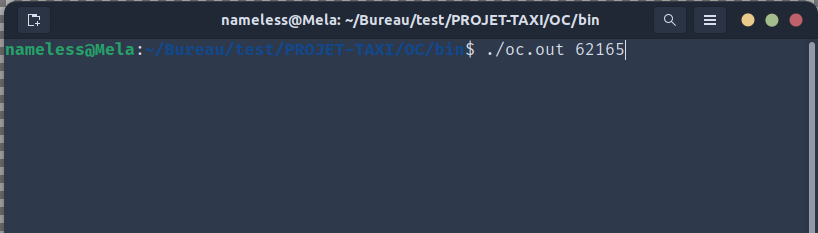
\includegraphics[width=1.0\textwidth]{Sections/Images/new_images/a400.png}
    \caption{compiling OC with pid of UI}
    \label{fig:enter-label}
\end{figure}

\begin{figure}[H]
    \centering
    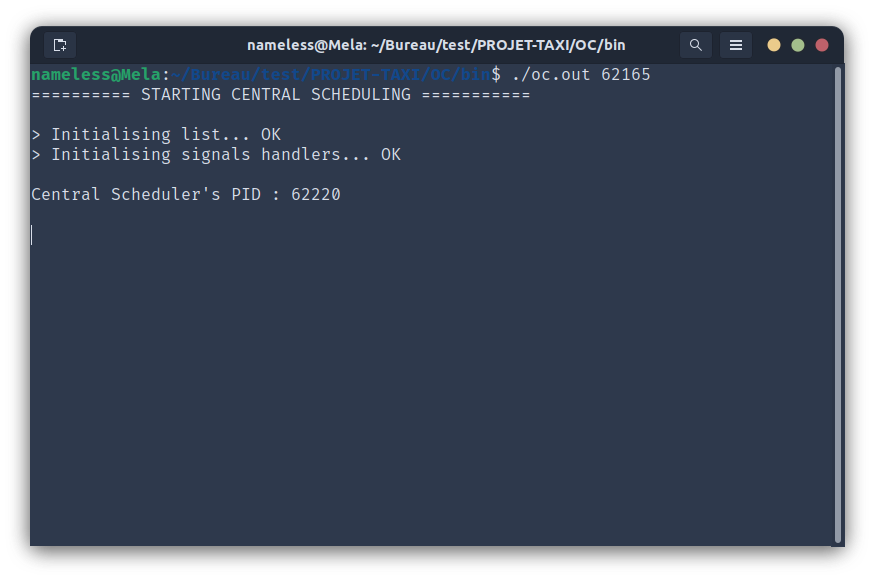
\includegraphics[width=1.0\textwidth]{Sections/Images/new_images/a5.png}
    \caption{result before the compilation of RPG}
    \label{fig:enter-label}
\end{figure}

\begin{figure}[H]
    \centering
    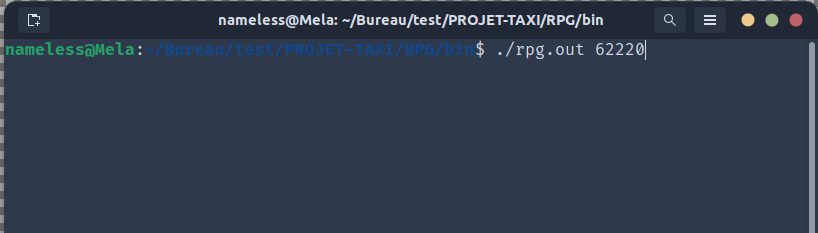
\includegraphics[width=1.0\textwidth]{Sections/Images/new_images/a600.png}
    \caption{compiling RPG with pid of OC}
    \label{fig:enter-label}
\end{figure}

% \begin{figure}[H]
%     \centering
%     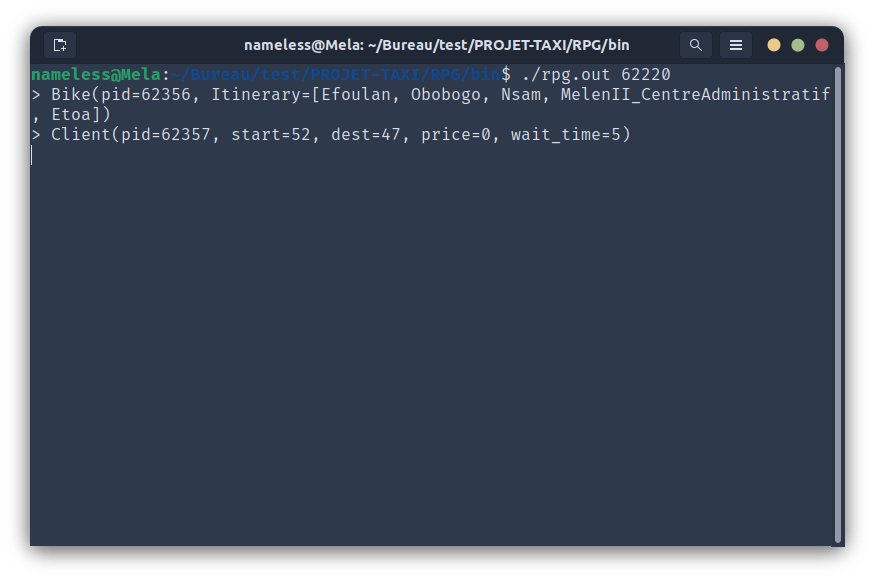
\includegraphics[width=1.0\textwidth]{Sections/Images/new_images/a7.png}
%     \caption{OC result}
%     \label{fig:enter-label}
% \end{figure}

\begin{figure}[H]
    \centering
    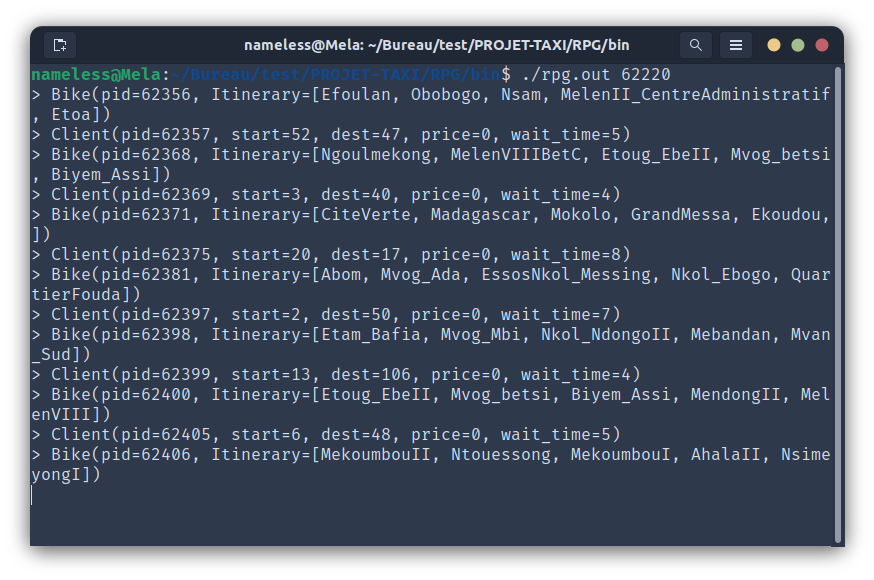
\includegraphics[width=1.0\textwidth]{Sections/Images/new_images/a8.png}
    \caption{RPG result}
    \label{fig:enter-label}
\end{figure}

\begin{figure}[H]
    \centering
    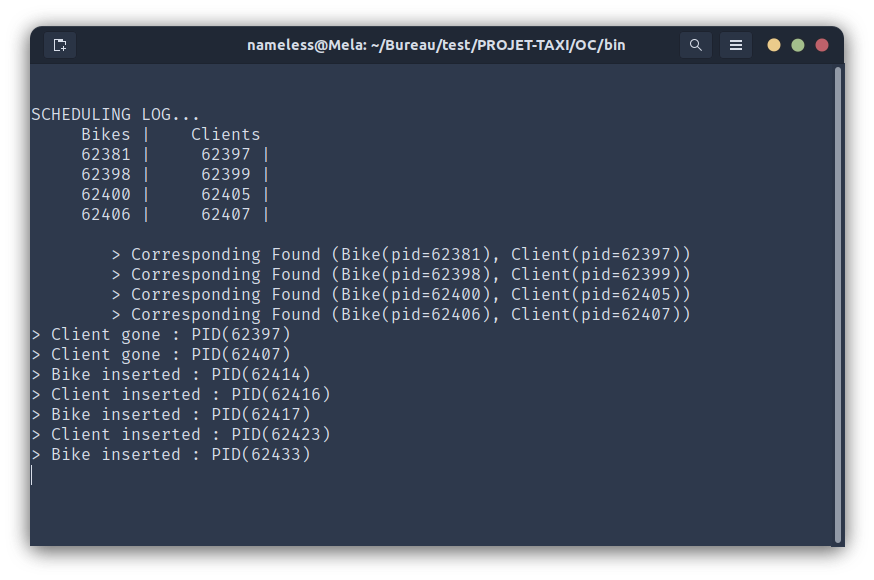
\includegraphics[width=1.0\textwidth]{Sections/Images/new_images/a9.png}
    \caption{OC result}
    \label{fig:enter-label}
\end{figure}

\begin{figure}[H]
    \centering
    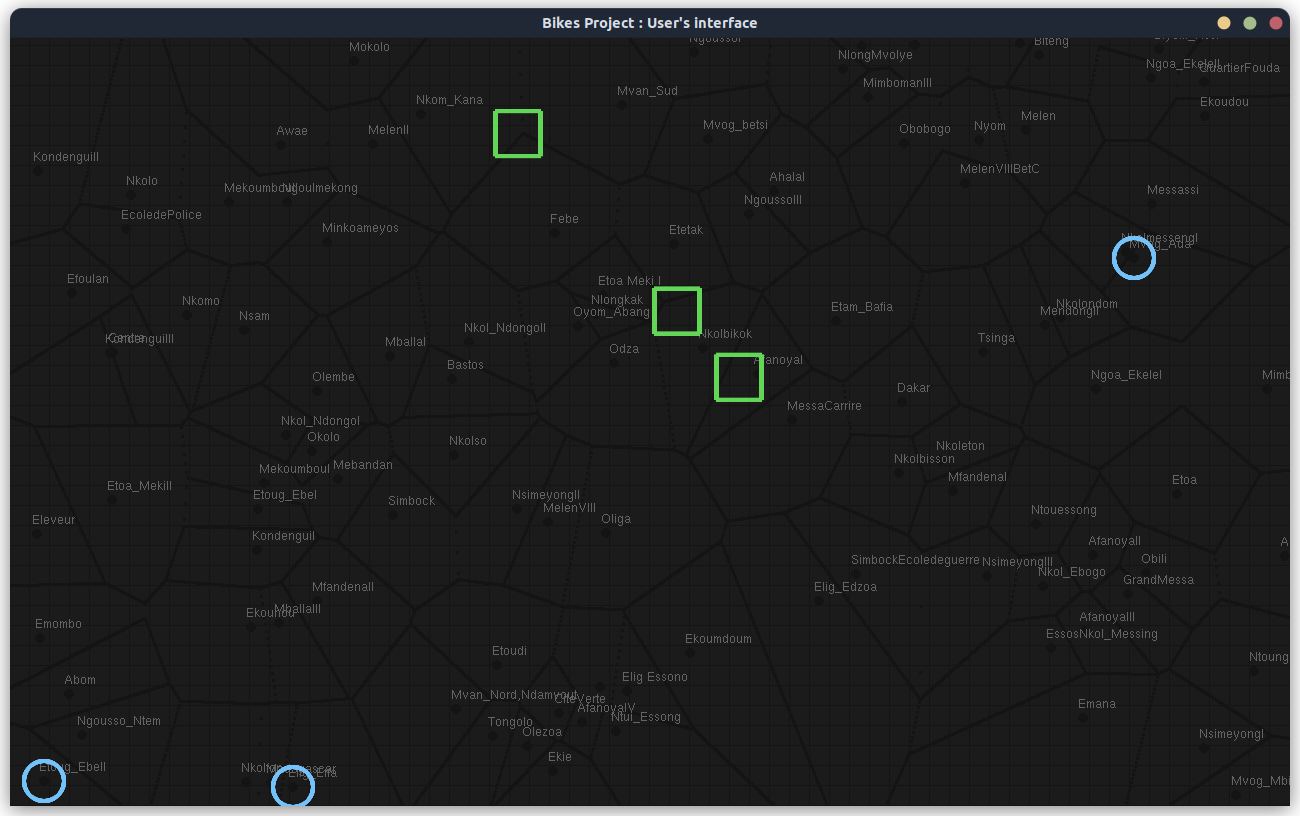
\includegraphics[width=1.0\textwidth]{Sections/Images/new_images/a10.png}
    \caption{interface result}
    \label{fig:enter-label}
\end{figure}

\begin{figure}[H]
    \centering
    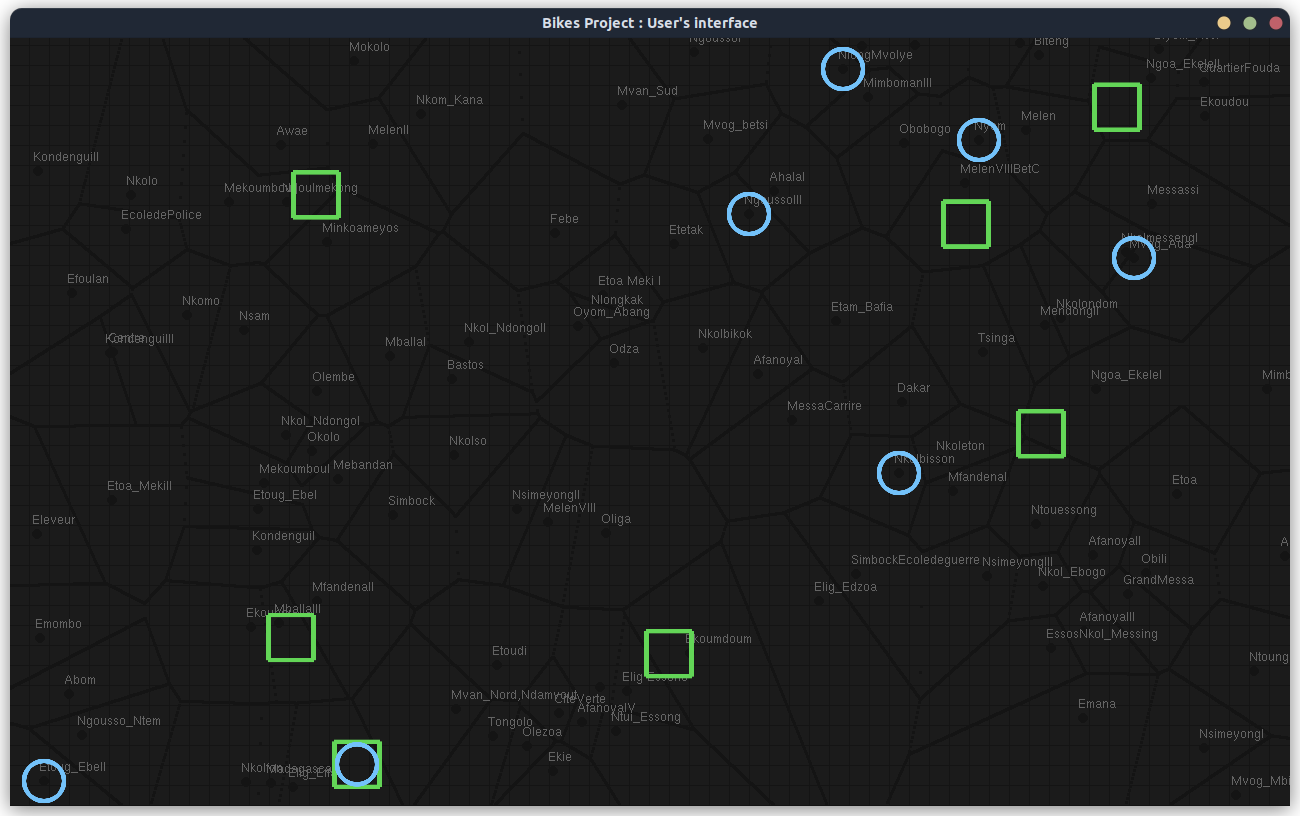
\includegraphics[width=1.0\textwidth]{Sections/Images/new_images/a11.png}
    \caption{interface result}
    \label{fig:enter-label}
\end{figure}

\begin{figure}[H]
    \centering
    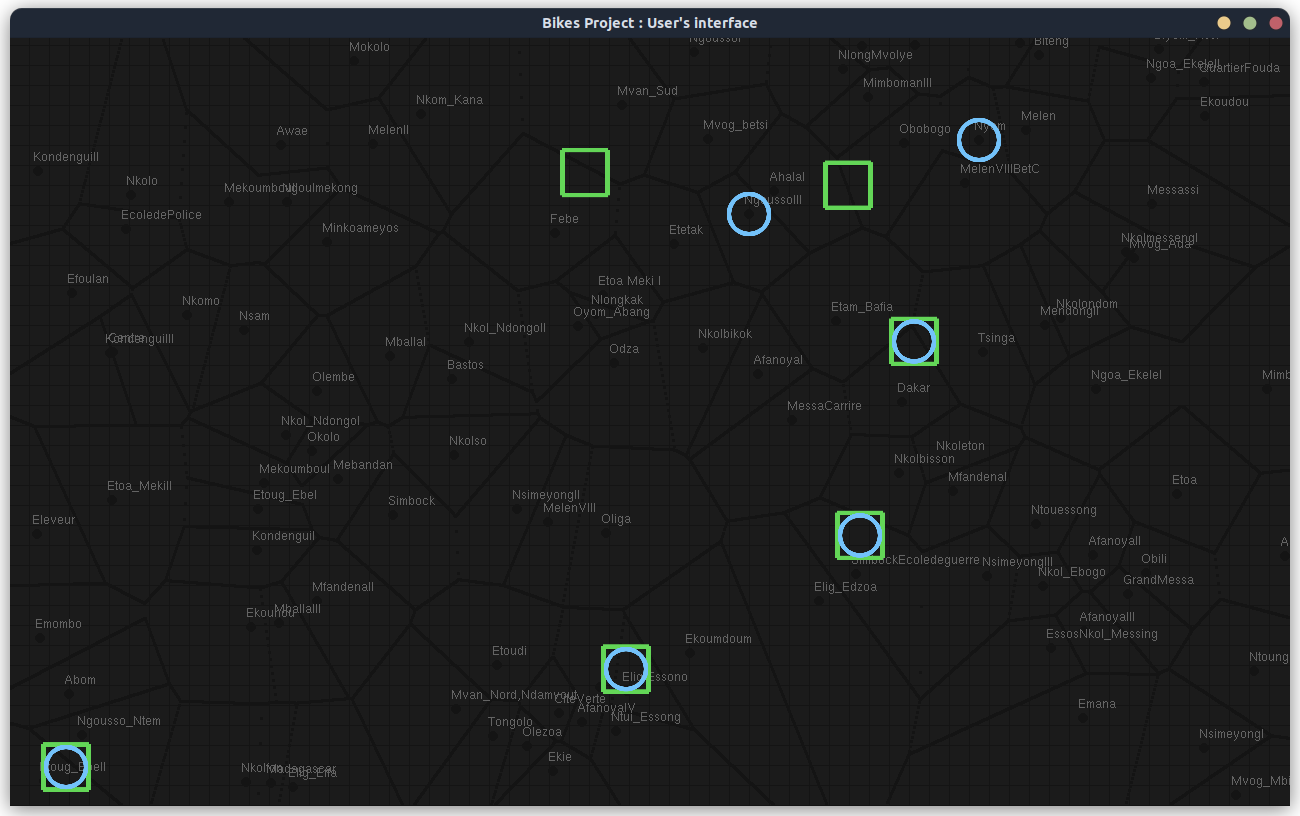
\includegraphics[width=1.0\textwidth]{Sections/Images/new_images/a12.png}
    \caption{interface result}
    \label{fig:enter-label}
\end{figure}

\begin{figure}[H]
    \centering
    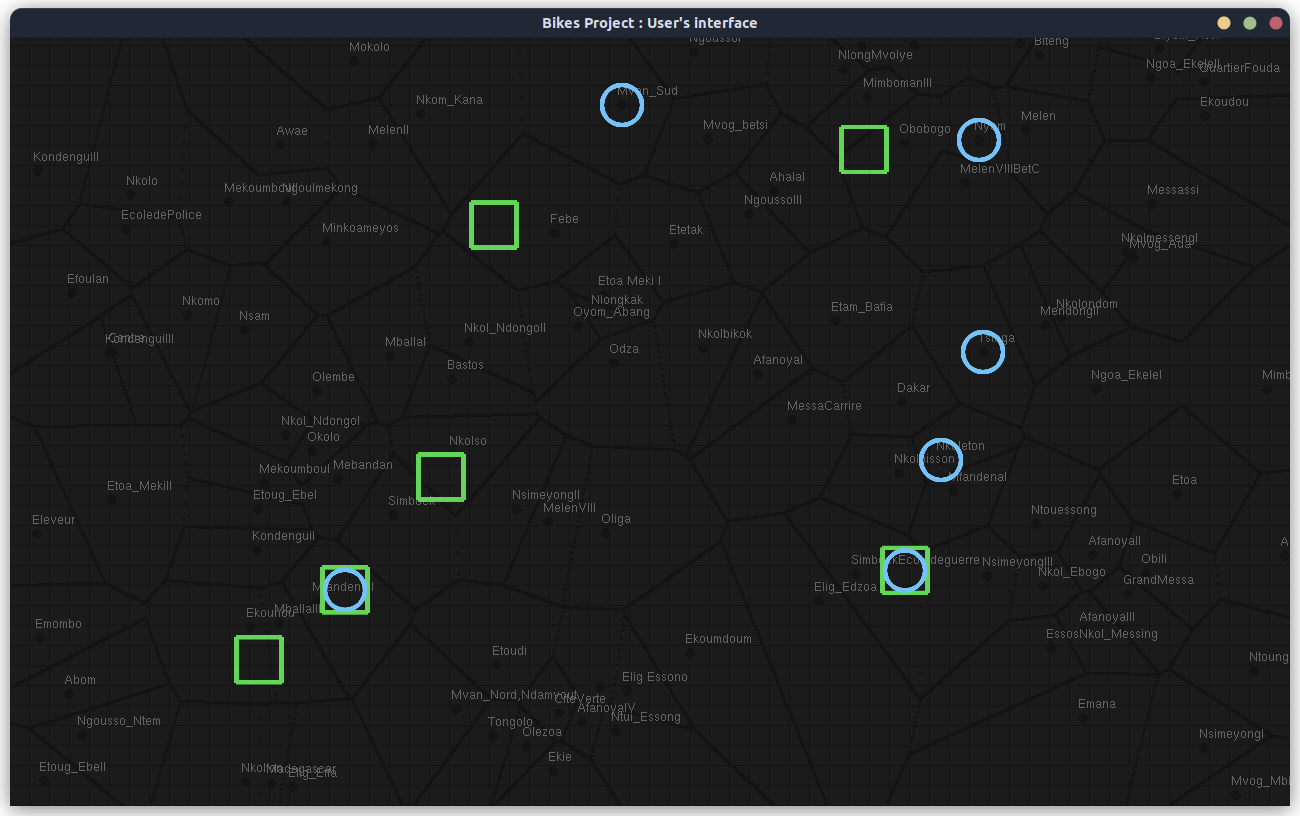
\includegraphics[width=1.0\textwidth]{Sections/Images/new_images/a13.png}
    \caption{interface result}
    \label{fig:enter-label}
\end{figure}

\newpage
\section{Conclusion}

In conclusion, the motorcycle project has addressed a significant challenge in the transportation domain, particularly for motorcycle taxis: the efficient pickup of clients. We recognized the importance of ensuring customer satisfaction by providing fast and reliable transport, and we have taken measures to achieve this.

We identified challenges associated with client pickups, including managing various parameters such as client locations and motorcycle availability. To address these challenges, we proposed developing a client pickup algorithm that adheres to a certain policy while simulating the operation of a motorcycle in real life.

Throughout this project, we posed crucial questions that guided our work and helped us define an appropriate policy and mode of operation for our motorcycle.

Ultimately, we believe that this project has the potential to transform the transportation sector. By offering fast and reliable service, we can not only meet the needs of our clients but also set new standards in the industry. We look forward to seeing how this project will evolve and contribute to enhancing the transportation experience for our clients. Thank you for accompanying us on this exciting journey.

\newpage

\end{document}
